\documentclass[12pt]{article}
% \usepackage[fontsize=12.2pt]{scrextend}
% Language setting
\usepackage[english]{babel}
\usepackage[
backend=biber,
style=apa,
citestyle=apa,
]{biblatex}

% Set page size and margins
% Replace `letterpaper' with `a4paper' for UK/EU standard size
\usepackage[letterpaper,top=2cm,bottom=2cm,left=3cm,right=3cm,marginparwidth=1.75cm]{geometry}

% Useful packages
\usepackage{amsmath}
\usepackage{graphicx}
\usepackage[colorlinks=true, allcolors=blue]{hyperref}
%\usepackage{caption}
\usepackage{subcaption}
\usepackage{doi}
\usepackage[font={scriptsize}]{caption}
\usepackage{authblk}
\usepackage{float}
\usepackage{appendix}
\usepackage{caption}
\usepackage{tocloft}
\usepackage{chngcntr}
\usepackage{forest}
\usepackage{listings}
\usepackage[dvipsnames]{xcolor}
\usepackage{hyperref}
\usepackage{multirow}
\usepackage{tabularx,colortbl}

\newcommand{\tocite}{\textcolor{red}{(CITE) }}

\hypersetup{
    colorlinks=true,
    linkcolor=black,
    urlcolor=blue,
    }

\usepackage[T1]{fontenc}
\usepackage{Alegreya} %% Option 'black' gives heavier bold face 

\definecolor{codegreen}{rgb}{0,0.6,0}
\definecolor{codegray}{rgb}{0.5,0.5,0.5}
\definecolor{codepurple}{rgb}{0.58,0,0.82}
\definecolor{backcolour}{rgb}{0.95,0.95,0.92}

\lstdefinestyle{mystyle}{
    backgroundcolor=\color{backcolour},   
    commentstyle=\color{codegreen},
    keywordstyle=\color{magenta},
    numberstyle=\tiny\color{codegray},
    stringstyle=\color{codepurple},
    basicstyle=\ttfamily\footnotesize,
    breakatwhitespace=false,         
    breaklines=true,                 
    captionpos=b,                    
    keepspaces=true,                 
    numbersep=5pt,                  
    showspaces=false,                
    showstringspaces=false,
    showtabs=false,                  
    tabsize=3
}

\lstset{style=mystyle}

\counterwithin{figure}{section}

\title{\vspace{-2cm} \Large Port Phillip Bay Wave-Hydrodynamic (SCHISM - WWM) Modelling}

\author[1]{\normalsize Franklin F. Ayala}
\author[1]{Huy Quang Tran}
\author[1,*]{Alexander V. Babanin}

\affil[1]{Faculty of Engineering and Information Technology (FEIT), University of Melbourne, Melbourne, VIC 3010, Australia; \href{mailto:a.babanin@unimelb.edu.au}{a.babanin@unimelb.edu.au}}

% \author{,  and  \\ Email address: }


\addbibresource{bibliography.bib} %Imports bibliography file

\begin{document}

\maketitle

\section*{Executive summary}
This report summaries  the work done in Stage 1 of the Wave-Hydrodynamic Modelling research project funded by the Department of Energy, Environment and Climate Action (DEECA). It focuses on updating the Port Phillip Bay  (PPB) wave-ocean hindcast datasets extented to 5 different SLR scenarios (0.0 m, 0.5 m, 0.8 m, 1.1 m and 1.4 m) and up to 32 years (1990-2021) using the state of the art wave physics (ST6) and the newly ERA5 atmospheric forcing field with the wind field locally scaled up to optimise the wave model performance which was validated against the operational wave buoy network recently deployed within the Bay.  From hourly modelled hindcast outputs, different percentiles and extreme levels were estimated for every grid point as well as  different contour lines (e.g. at different water depth or different distance to the shoreline). It is expected that this  dataset would be an useful resource for various applications within PPB in the year to come.  Although every effort has been made to produce a high quality hindcast dataset up to present time, it is also possible that a new version of this dataset will be made available when there is a new or an improved atmospheric product released to the public (e.g. ERA 6).\\


% The Port Phillip Bay (PPB) is arguably one of the most important environmental, social and economic asset in Victoria. In this study, the efforts to improve hydrodynamic climate of PPB is shown with the aid of a coupled high-resolution wave-current numerical modelling system (SCHISM-WWM) using advanced wave physics, the latest ERA5 atmospheric products as forcing conditions and a real-time observational buoy network recently deployed in PPB. The validation results indicate a good agreement between the model and the buoy measurements, even for the most extreme wave event in PPB, where the observed significant wave height $H_s$ exceeded 3.5 m at Mt Eliza. Further, long-term simulations under different sea level scenarios were conducted to hindcast sea state conditions for 32-years period (1990-2021) based on the newly validated modelling system. This data has been used to carried out extreme value analysis (EVA) to estimate 500-,100-,50-, and 20-year return levels of variables such as $H_s$, elevation and current speed for different locations within PPB according to the Victoria’s Resilient Coast guidelines.\\

\noindent
\textbf{Keywords}: Port Phillip Bay, coupled hydrodynamic model, extreme value analysis


\newpage

\tableofcontents

\newpage

\listoffigures

\newpage

\hypersetup{
    colorlinks=true,
    linkcolor=blue,
    urlcolor=blue,
    }

\section{Introduction}

A broadly-used regional scale wave model is employed in Port Phillip Bay (PPB) to analyse the wave damping due to bottom dissipation and vegetation. This is an vital step to quantify the effect of the bottom conditions and habitat types in PPB and finally to represent enough accurately the wave climate across the bay. The University of Melbourne (UoM) has previously developed a coupled wave-hydrodynamic model (SCHISM-WWMIII) of PPB, through Dr. Huy Tran as a part of his PhD research, supervised by Prof. Alex Babanin, in collaboration with the Victorian Coastal Monitoring Program. Despite these advances, bottom friction physics (e.g. generation of ripples and its drag mechanism) and the interaction wave-current under vegetation cases are not completely implemented in SCHISM-WWMIII yet, which leads to the use of the Simulation WAves Nearshore (SWAN) model and its coupling with the Regional Ocean Modelling System (ROMS). Since Dec 2020, a network of wave buoys were deployed across the Bay as part of the Victorian Coastal Monitoring Program. It is now possible to produce an updated PPB wave model, utilising the wave buoy observations. The proposed project will take advance of the emerged numerical modelling and the newly available in-situ observation to:

\begin{itemize}
    \item Evaluate a more realistic bottom friction conditions in the wave damping for PPB.
    \item Assessing the impact of the vegetation in the wave propagation for some areas of the bay.
    \item Implementing a regional coupled wave-current simulation to include the effect of the vegetation in the ocean currents/sea level in PPB.
\end{itemize}

% Port Phillip Bay (PPB) is a dynamic system that covers approximately 1,934 km$^{2}$ and has 333 km of shoreline serving various human interests, including fishing, recreational activities, and ship navigation in Victoria (see Fig. \ref{fig:study_zone}). PPB has a tidal inlet system connected with a narrow entrance (a mere 3km wide) on the southern side where the bathymetry is very steep. Specifically, there is a deep and narrow canyon $>$ 90m deep and 150m wide, curved by relatively shallow regions where the water depth falls below 20m. Towards the inner bay, there is a main navigational channel system that dissects the shallow inlet region into two parts, featuring a sand island and many sand bars. Outside the inlet system, there is also a shallow C-curved region called the offshore bar. The entrance of PPB (Port Phillip Head [PPH] or simply the Heads) also exhibits energetic waves that propagate from the Southern Ocean and interact with strong inverse tidal currents all year around.

% \begin{figure}[h]
% \centering
% \begin{minipage}{.5\textwidth}
%   \centering
%   \includegraphics[width=\linewidth]{study_zone.png}
%   \captionof{figure}{Study zone}
%   \label{fig:study_zone}
% \end{minipage}%
% \begin{minipage}{.5\textwidth}
%   \centering
%   \includegraphics[width=0.75\linewidth]{buoy_locations.png}
%   \captionof{figure}{Location of the buoy measurements in PPB}
%   \label{fig:buoy_measurements}
% \end{minipage}
% \end{figure}

% The natural features of tidal inlets in PPB have been disrupted by
% engineering modifications. In particular, a capital dredging project was carried out
% in PPB during 2008 - 2009 as part of a port upgrade to serve larger vessels up to
% 7,000 TEU with 14m draught by 2035 at all tidal conditions. The major works
% were carried out within the south channels. In this region, the channel system was
% environmentally deepened by up to 3m \parencite{MinPLanning}.

\section{Methodology}

\subsection{Numerical modelling framework}

\subsubsection*{Wave model}

SWAN is a numerical model designed for simulating coastal wave dynamics that propagates the wave energy based on the wave action balance equation with sources and sinks using a spectral wave approach, allowing for detailed representation of wave energy across frequencies and directions. Notably, SWAN captures the nonlinear interaction between waves and wind, essential for accurately modelling coastal wave behaviour. It also accounts for shallow-water effects, including wave shoaling and refraction and it can be coupled with hydrodynamic models to study wave-current interactions, providing a comprehensive understanding of coastal processes. The model supports various boundary conditions and flexible grid systems, accommodating different coastal geometries and its reliability is backed by extensive validation against experiments and field measurements. Overall, SWAN is a valuable tool for coastal engineers, researchers, and decision-makers involved in coastal management, offering accurate simulations of complex coastal wave dynamics.

For the simulations in PPB, the depth-induced breaking was activated \parencite{Battjes1978}, the third-generation physics were also used. Different dissipation expressions by bottom friction were tested \parencite{Madsen_Poon_Graber_1988,Smith2011} and vegetation damping \parencite{Suzuki2011} was also included in some of the runs.

\subsubsection*{Ocean-wave model}

The current-wave interaction is intended to be studied using the modelling system COAWST \parencite{Warner2010}, an open-source model that combines many sophisticated systems that each provide relative earth-system components necessary to investigate the dynamics. Specifically, the COAWST Modeling System includes an ocean component—Regional Ocean Modeling System (ROMS); atmosphere component—Weather Research and Forecast Model (WRF), hydrology component- WRF\textunderscore Hydro; wave components—Simulating Waves Nearshore (SWAN), WAVEWATCHIII, and InWave; a sediment component—the USGS Community Sediment Models; and a sea ice model.

\begin{figure}[h]
    \centering
    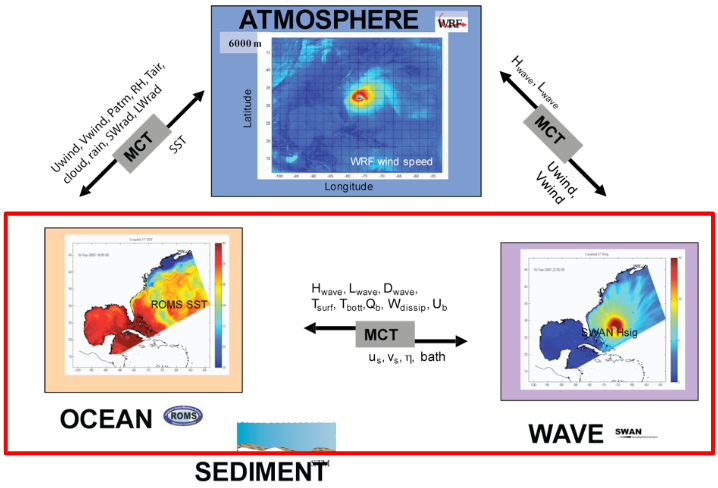
\includegraphics[scale=0.7]{plots/coawst_structure.PNG}
    \caption{Diagram with the model components of COAWST. The components used in this study are within the red box. The coupling variables are also depicted.}
    \label{fig:coawst_structure}
\end{figure}

The vegetation module...

\begin{figure}[h]
    \centering
    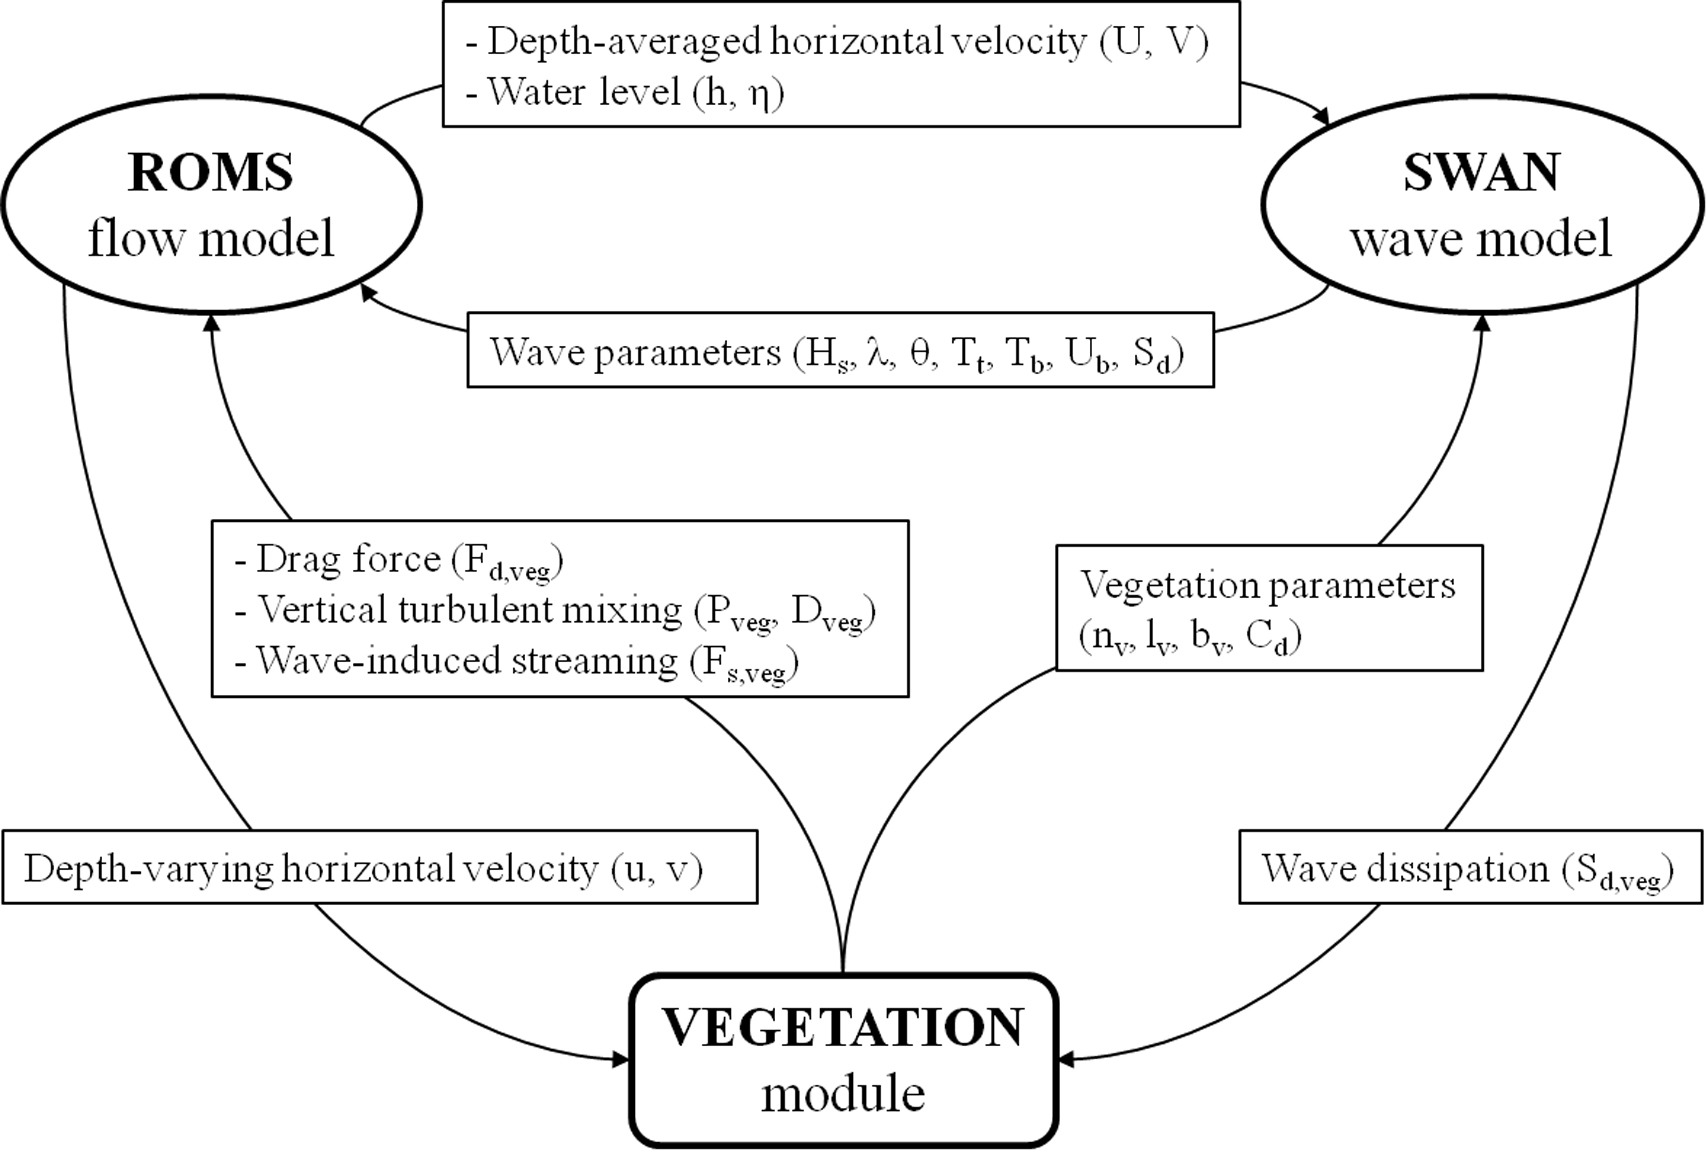
\includegraphics[scale=1.1]{plots/scheme_vegetation_module.jpg}
    \caption{Scheme of the vegetation module implemented in COAWST modelling system.}
    \label{fig:scheme_vegetation_module}
\end{figure}

\subsection{Model setup} \label{sec:model_setup}

\subsubsection{Bathymetric processing}

Bathymetry datasets were gathered from several sources at different resolutions ranging from 0.5 to 500 m. Within the southern area of PPB, including the entrance, bathymetry data were mainly measured via LADS surveys with a high resolution (up to 6 m). These bathymetric measurements were taken during summer 2007/2008 (before channel deepening) and summer 2009/2010 (after channel deepening). Along shipping channels, the bathymetry after dredging was measured by MBES with a 0.5 m resolution in a rectangular grid format. These high-resolution data used MGA94 (Zone 55) map projection. For other areas within PPB, bathymetry was taken from the Victorian coastal digital elevation model (VCDEM 2017) with a 500 m resolution. The bathymetry data was combined into a single set that covers the whole domain, and the information recorded in MGA94 projections within the southern region of PPB was converted into WGS84 projections to unify the coordinate system. The bathymetry can be visualized in the figure \ref{fig:bathy_PPB}.

\subsubsection{Computational mesh}

A curvilinear grid was used for all the simulation with 99 meshes in $\xi-$direction and 199 meshes in $\eta-$direction (see figure \ref{fig:grid_PPB}). This grid covers all the bay and initially its open boundary is extended further from the entrance of the bay into deep waters (approximately 70 m deep). This extension allows capturing waves from deep waters.

\begin{figure}[h]
\centering
\begin{subfigure}{.5\textwidth}
  \centering
  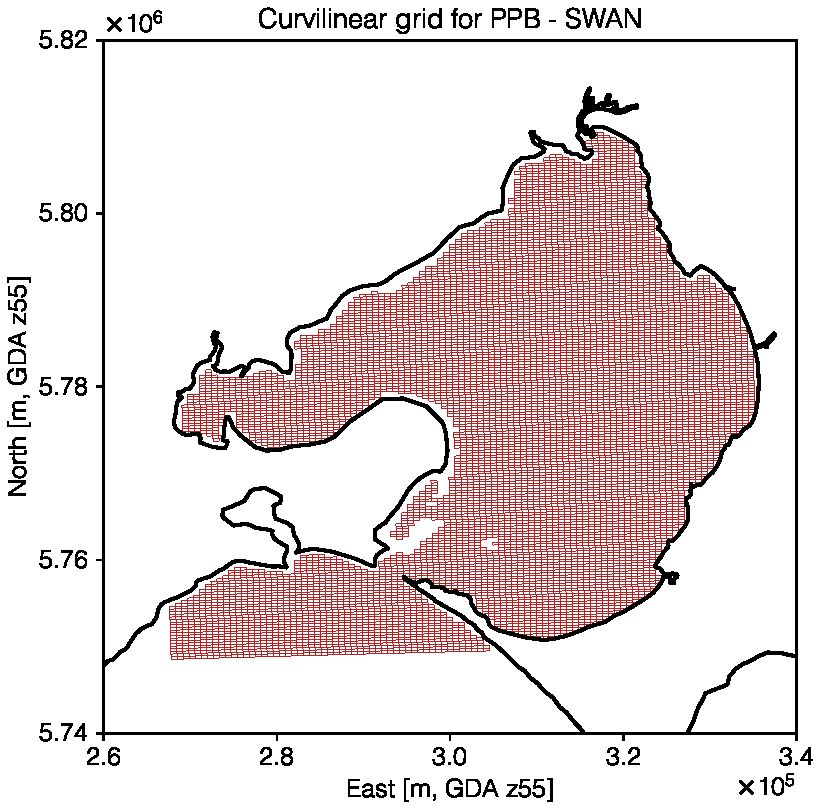
\includegraphics[scale=0.55]{plots/maps/grid_SWAN.pdf}
  \caption{Curvilinear grid employed in SWAN for PPB}
  \label{fig:grid_PPB}
\end{subfigure}%
\begin{subfigure}{.5\textwidth}
  \centering
  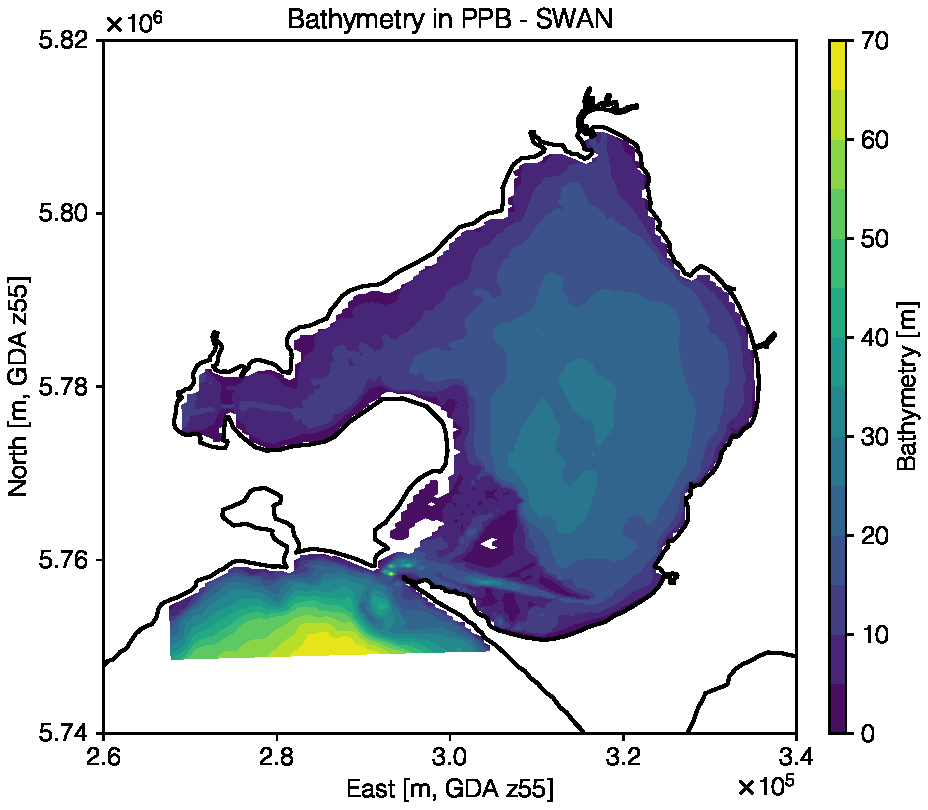
\includegraphics[scale=0.55]{plots/maps/bathymetry_SWAN.pdf}
  \caption{Bathymetry used for SWAN for PPB}
  \label{fig:bathy_PPB}
\end{subfigure}
\caption{Visualisation of the final mesh and bathymetry used in this study}
\label{fig:grid_bathy_PPB}
\end{figure}

\subsubsection {Model Forcing}

Coastal models are typically applied for a region in contact with external regions via the open boundary. Therefore, the open boundary conditions should be specified. The following sections describe the types of forcing required to run SWAN and ROMS.

\subsubsection*{Elevations/tidal forcing}

For coastal wave-current interaction modelling, the water level has to be specified across both time and space. In practice, at the very least, these water elevations (or tidal velocities) are then used to force the circulation model to capture the feedback between the waves and currents. To specify the tides across the domain, this study used the tidal constants computed from TPXO 8 Atlas data \parencite{Egbert2002} for the simulation period. The method used is harmonic analysis and the astronomic tides are constructed based on the registered harmonics.  

\subsubsection*{Atmospheric forcing}

In this study, the atmospheric forcing inputs for SCHISM/WWM were derived from the reanalysis ERA5 products \parencite{Hersbach2019}. It is the fifth generation ECMWF atmospheric reanalysis of the global climate, covering the period from January 1940 to present. ERA5 is produced by the Copernicus Climate Change Service (C3S) at ECMWF. ERA5 provides hourly estimates of various atmospheric, land and oceanic climate variables. The data cover the Earth on a 30 km grid and resolve the atmosphere using 137 levels from the surface up to a height of 80 km. The wind forcing was downloaded from 0000 01-Oct-2021 to 2300 06-Nov-2021. 

\subsubsection*{Bottom conditions}

The grain diameter size is available in a cloud point for PPB. This data is formatted in phi scale as it can seen in the figure \ref{fig:diameter_phi} and it can be easily translated into a millimetre scale (fig. \ref{fig:diameter_mm}) using the equation:

\begin{equation}
    \phi = - \log_{2}\frac{D}{D_0}
\end{equation}

where $D_0$ is the standard diameter size equals to 1 mm and $D$ is the diameter in mm. This information has to be converted into mm in order to prepare the diameter size in a conventional measurement system that SWAN can read.

\begin{figure}[h]
\centering
\begin{subfigure}{.5\textwidth}
  \centering
  \includegraphics[scale=0.45]{plots/maps/sediment_distribution_phi.png}
  \caption{Diameter grain size distribution in PPB [$\phi$ scale]}
  \label{fig:diameter_phi}
\end{subfigure}%
\begin{subfigure}{.5\textwidth}
  \centering
  \includegraphics[scale=0.45]{plots/maps/sediment_distribution_mm.png}
  \caption{Diameter grain size distribution in PPB [mm]}
  \label{fig:diameter_mm}
\end{subfigure}
\caption{Conversion of the diameter grain size distribution in PPB from the $\phi$ to mm scale }
\label{fig:diameter_PPB}
\end{figure}

The highest values of diameter size are in the centre of the bay (close to 1 mm). \textcolor{red}{a brief description of that}

Because of the grain size data resolution neither does not match with the SWAN computation grid nor it is not regular, the information was spatially interpolated into a rectangular grid for PPB. A python script was made to build the regular grid from the cloud point in function of an initial point, horizontal resolution $dx$ and vertical resolution $dy$.

\begin{figure}[h]
    \centering
    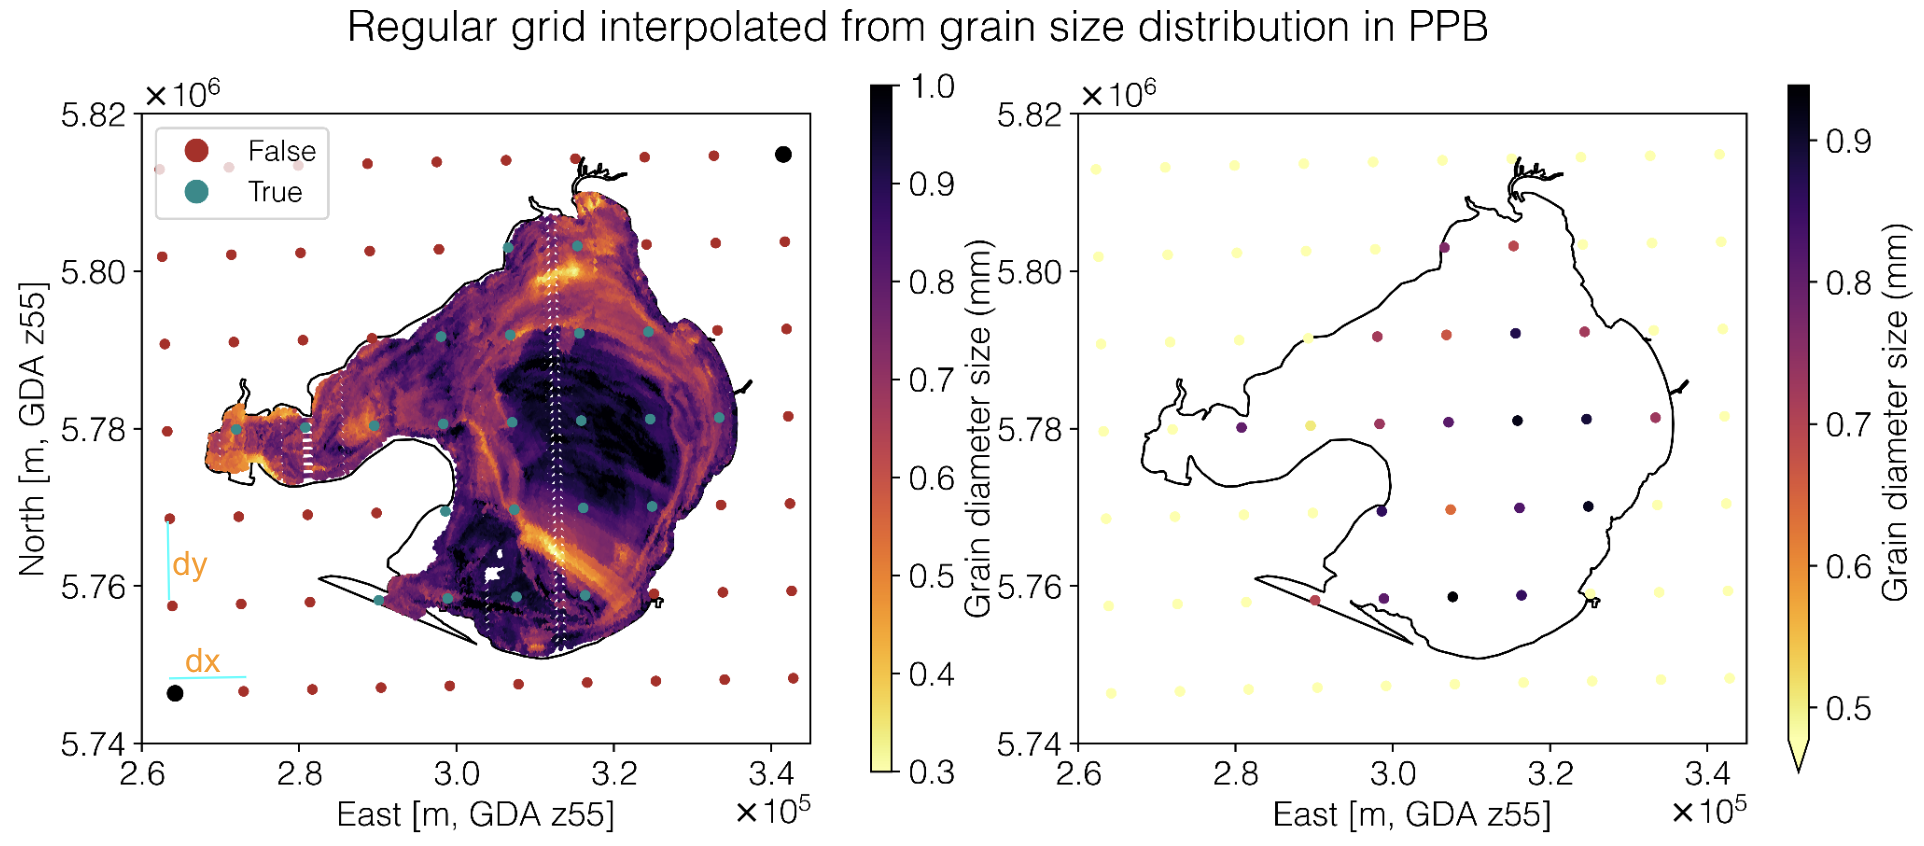
\includegraphics[scale=0.45]{plots/maps/interpolated_D.png}
    \caption{Regular grid interpolated from grain size distribution in PPB. On the left panel the points inside the bay are dark cyan while the outer ones are red. The interpolated points inside PPB are shown in function of its diameter value on the right panel}
    \label{fig:interpolated_D}
\end{figure}

On the left panel in the figure \ref{fig:interpolated_D} an initial partitioning of the points based on whether they are inside on the bay or not. The points outside PPB are defined as \verb|NaN| values and the inner ones are spatially interpolated based on the neighbour locations as it shown in the right panel. The $dx$ and $dy$ are chosen for illustrative purposes, but a finer resolution (e.g. 0.01 degrees) can be selected as it be required.

\subsubsection*{Vegetation}

On top of the bottom grain size, the vegetation habitat types in PPB are also available. The sublittoral sand and sublittoral mud are the most dominant habitats in the area (see fig. \ref{fig:sg_PPB}) and other ecosystems like sublittoral seagrass beds are also prominent in Corio Bay, Swan Bay and Queenscliff.

\begin{figure}[h]
    \centering
    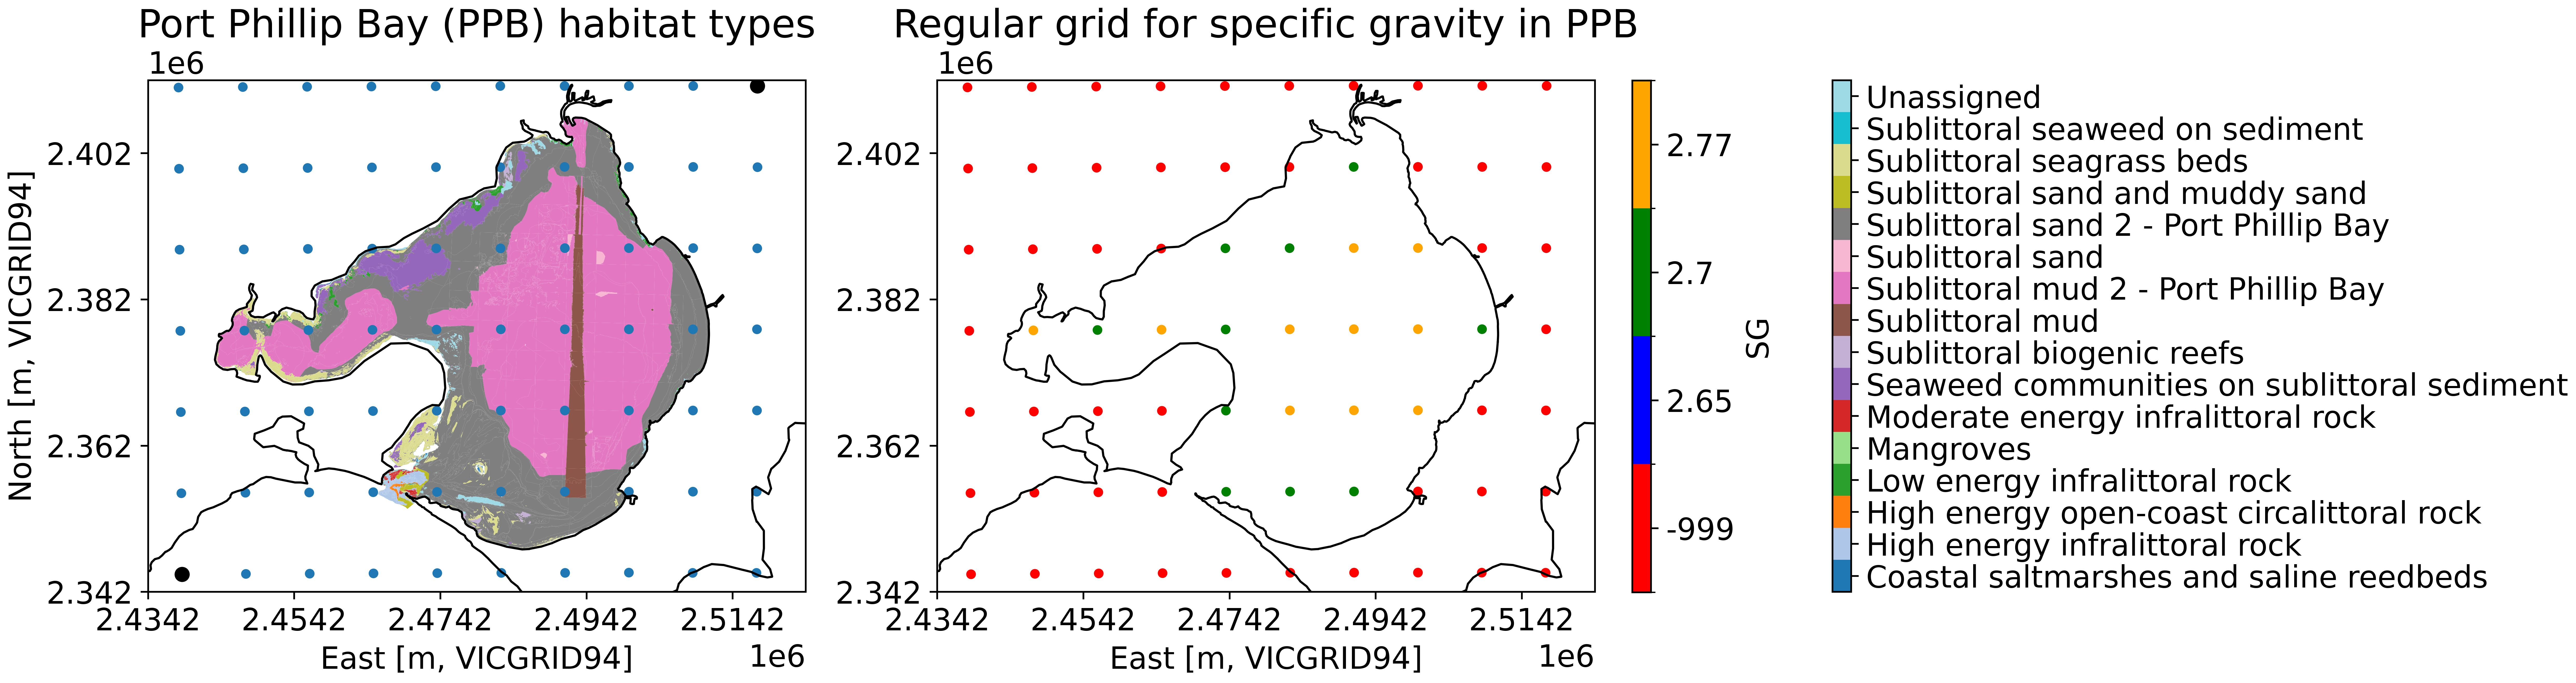
\includegraphics[scale=0.4]{plots/maps/PPB_habitat_types_0.1_0.1.png}
    \caption{Habitat types and regular grid for specific gravity (SG) in PPB}
    \label{fig:sg_PPB}
\end{figure}

All the attributes for the habitat type data are assigned in polygons and they had to be converted into a regular grid as well. The specific gravity for those habitat types was then interpolated from the polygons to a regular grid due to it is used as an input variable in the \textcite{Smith2011} parametrization to compute the ripples in the wave dissipation by bottom friction. For the interpolation, different specific gravity values were assigned into the polygons accordingly with the habitat type (mud, sand, seaweed, sea grass, etc.). Each habitat type can even has its corresponding specific gravity range and therefore it is difficult determining a unique value of specific gravity, for example this variable for mud can range from 2.65 to 3.4. Additionally, there are some habitat types (i.e. related with vegetation) which have no clear information about their specific gravity like mangroves, sea grass, seabed, infralittoral rock, among others.\\

Clearly, describing the bottom friction and the specific gravity across the bay is more physically reliable/representative than just assigning a singular value for these variables for the entire area.

\subsection{Experiments}

In order to check the SWAN performance under different bottom friction parametrizations and to get the most physic reliable configuration, a set of experiments was purposed:

\begin{table}[h]
\begin{tabular}{|c|c|c|c|c|}
\hline
\rowcolor{orange}
Experiment name & \begin{tabular}[c]{@{}c@{}}Bottom friction \\ parametrization\end{tabular} & \begin{tabular}[c]{@{}c@{}}Diameter size\\ D (mm)\end{tabular} & \begin{tabular}[c]{@{}c@{}}Specific gravity\\ SG\end{tabular} & \begin{tabular}[c]{@{}c@{}}roughness \\ kn (m)\end{tabular} \\ \hline
madsen            & \textcite{Madsen_Poon_Graber_1988}                  & N/A                   & N/A          & 0.05            \\ \hline
smith s2.65 d0.1  & \textcite{Smith2011}             & 0.1                   & 2.65         & N/A       \\ \hline
smith s2.65 d0.78 & \textcite{Smith2011}             & 0.78                  & 2.65         & N/A       \\ \hline
smith s2.65 d0.01 & \textcite{Smith2011}             & 0.01                  & 2.65         & N/A       \\ \hline
smith 2.75 d0.01  & \textcite{Smith2011}             & 0.01                  & 2.75         & N/A       \\ \hline
smith s2.65 dvar  & \textcite{Smith2011}             & Spatial variable      & 2.65         & N/A       \\ \hline
\end{tabular}
\caption{Summary of the bottom friction configurations used in the experiments for PPB}
\end{table}

It has to be mentioned that \textcite{Madsen_Poon_Graber_1988} and \textcite{Smith2011} are dependent on different parameters. The key variable in \textcite{Madsen_Poon_Graber_1988} is an equivalent roughness length scale of the bottom, kn whom default value is 0.05 m. In \textcite{Smith2011} the two main variables are the specific gravity and the diameter grain size and their default values are 2.65 and 0.1 mm, respectively.

\subsection{Buoy measurements}

Victorian Coastal Monitoring Program (VCMP) deployed SOFAR Spotter buoys to measure the wave motions at sites along the perimeter and centre of PPB, as shown in Figure \ref{fig:buoy_measurements}. This real-time buoy network is part of the effort made by the Victorian government to understand how the deep water waves are transformed as they approach the shore and to develop a downscaling of models to associate wave climate with shoreline dynamics. The buoys record the rise and fall of the water surface approximately every half a second, use GPS positioning, transmit their data via satellite. The locations/labels of the buoys are: Werribee, Sandringham, Indented Head, Rosebud, Mt. Eliza, and Central PPB and they are recording wave variables such as SWH, peak direction, peak period, and mean period. These recorded variables were used to calibrate and validate the coupled modelling system to generate the long-term hindcast series in PPB.

\begin{figure}[h]
\centering
  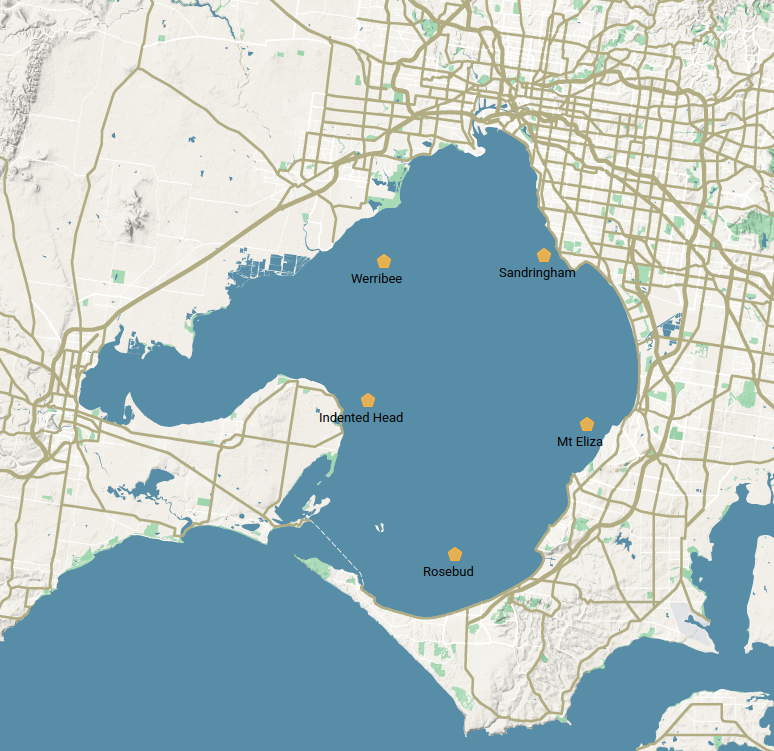
\includegraphics[scale=0.3]{plots/maps/vicwaves_buoy_locations.png}
  \caption{Location of the buoy measurements in PPB. Extracted from \url{https://vicwaves.com.au/}.}
  \label{fig:buoy_measurements}
\end{figure}

The buoy data were pre-processed prior to be used during the calibration/validation stage, since irregular movements and moorings can generate physically unreasonable measurements in the real-time buoy network in PPB. The fast-changing periods of the measured variables along the time series are used to identify the unrealistic measurements.\\

Figure \ref{fig:pre_processing} shows the  measured $H_{s}$ time series  from each buoy in the raw format (blue line) and in the despiked format (or without noises) (orange line). Note that the Sandringham, Rosebud, Indented Head, and central PPB stations had at least one spike, but all of them were removed in the final $H_{s}$ time series.  All the buoys show a good agreement within the storm events. Mt. Eliza and Sandringham stations registered the highest $H_{s}$ values among all the datasets.

\begin{figure}[h]
    \centering
    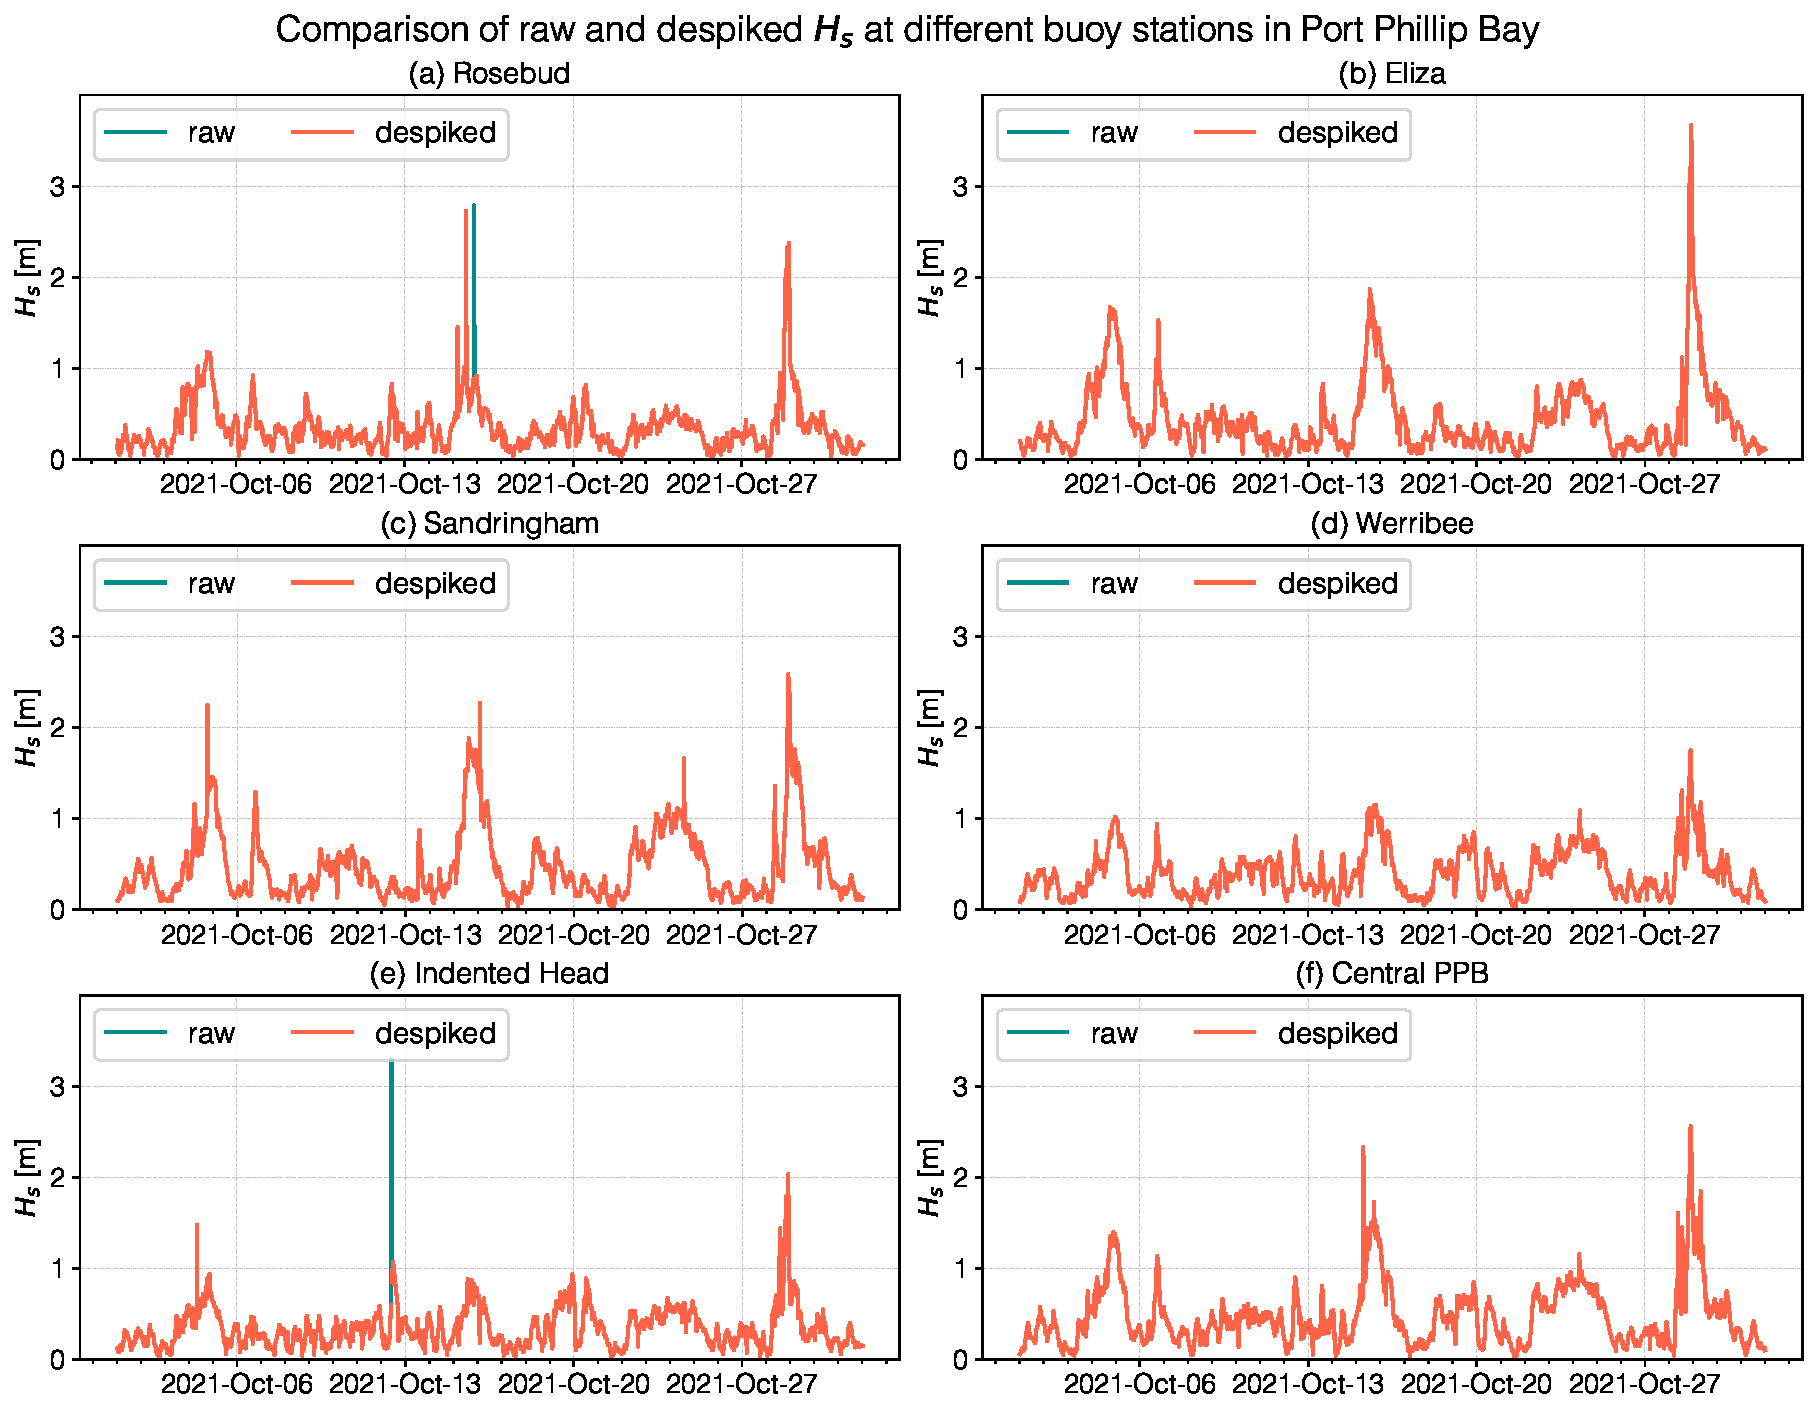
\includegraphics[scale=0.5]{plots/maps/buoy_despiked.pdf}
    \caption{Comparisons of the raw and processed (despiked) $H_{s}$ time series for each buoy location in PPB.}
    \label{fig:pre_processing}
\end{figure}

\subsection{Model calibration and validation}

An initial simulation for one-month period (from 01/10/2021 to 01/11/2021) was conducted with the purpose of validating the wave model against buoy observations. Those previous results showed an overall overestimation of $H_{s}$ at most of the buoy locations. Additionally, the wave height was underestimated by the model at the Mt. Eliza station during a storm event on October 28, 2021.

% A second simulation was carried out over the same period of time, with no scaling factor applied to the wind speed used in the model. This modification improved the estimation of the $H_{s}$ values in each buoy in comparison with the wind scaling factor simulation, but $H_{s}$ values for most buoys remained overestimated as well as the underestimation of the storm event recorded in Mt. Eliza in late October.

% Although overestimations of $H_{s}$ mean an underperformance of the modelling system, they do not represent a safety issue by comparison to the underestimations of storm events (e.g. Mt. Eliza buoy), therefore the main focus at this stage was on the enhancement of estimation of the events that were underestimated during the simulation period. In order to address this, a set of experiments were conducted. First, an experiment was performed to verify whether the waves generated by offshore were well represented by the model at Mt. Eliza. Secondly, experiments with changes of the main parameters of the dissipation, wind input, and bottom friction parametrizations used in the model to simulate the waves were developed, and finally, a local wind adjustment was done at grid points in the vicinity of the Mt. Eliza buoy.

% The best performance was obtained under the configuration of the localised wind scaling experiment. Figure \ref{fig:regional_wind_scaling} shows a better agreement between the high $H_{s}$ values registered by the Mt. Eliza buoy and estimated by the model.

% \begin{figure}[p]
%     \centering
%     \includegraphics[scale=0.7]{regional_wind_scaling.pdf}
%     \caption{$H_{s}$ time series for each buoy under the regional wind scaling experiment.}
%     \label{fig:regional_wind_scaling}
% \end{figure}

% As shown in Figure \ref{fig:qqplot}, RMSE is lower than 0.26 m at all the stations, and the negative mean bias per buoy demonstrates the overall model overestimation mentioned before. The best performance of the model was reported in the Sandringham station, while at the Rosebud station the highest overestimation of $H_{s}$ was recorded. This model configuration was then used for hindcast, including in the different sea level scenarios.

% \begin{figure}[p]
% \centering  
%   \includegraphics[scale=0.9]{model_vs_buoy.pdf}
%   \caption{Comparison between modelled and observed $H_{s}$ values for each buoy.}
%   \label{fig:qqplot}
% \end{figure}

\newpage

\section{Simulations results about different bottom friction}

Initially the experiments \textbf{madsen} and \textbf{smith s2.65 d0.1} were compared to have a general perspective of the model performance for the simulation period. 

\begin{figure}[H]
    \centering
    \includegraphics[scale=0.7]{plots/hs_series/madsen_vs_smith s2.65 d0.1_vert.png}
    \caption{$H_{s}$ time series for each buoy under madsen (pink line) and smith s2.65 d0.1 (cyan line) experiments.}
    \label{fig:hs_madsen_vs_smith_def}
\end{figure}

Both experiments represent correctly the $H_s$ variability along the simulation period, however, the maximum $H_s$ events are still underestimated by the model. Although the peaks are better estimated with \textbf{smith s2.65 d0.1} than \textbf{madsen}, there are differences between 0.5m and 0.8m between the largest simulated and measured $H_s$ per each station. Mt Eliza is the only station with $H_s$ values over 3m and it exhibits the highest $H_s$ event of 3.67 m, this event was not enough well captured by the model which represented 3.18 and 3.13 with \textbf{smith s.65 d0.1} and \textbf{madsen}, respectively.

\begin{figure}[H]
    \centering
    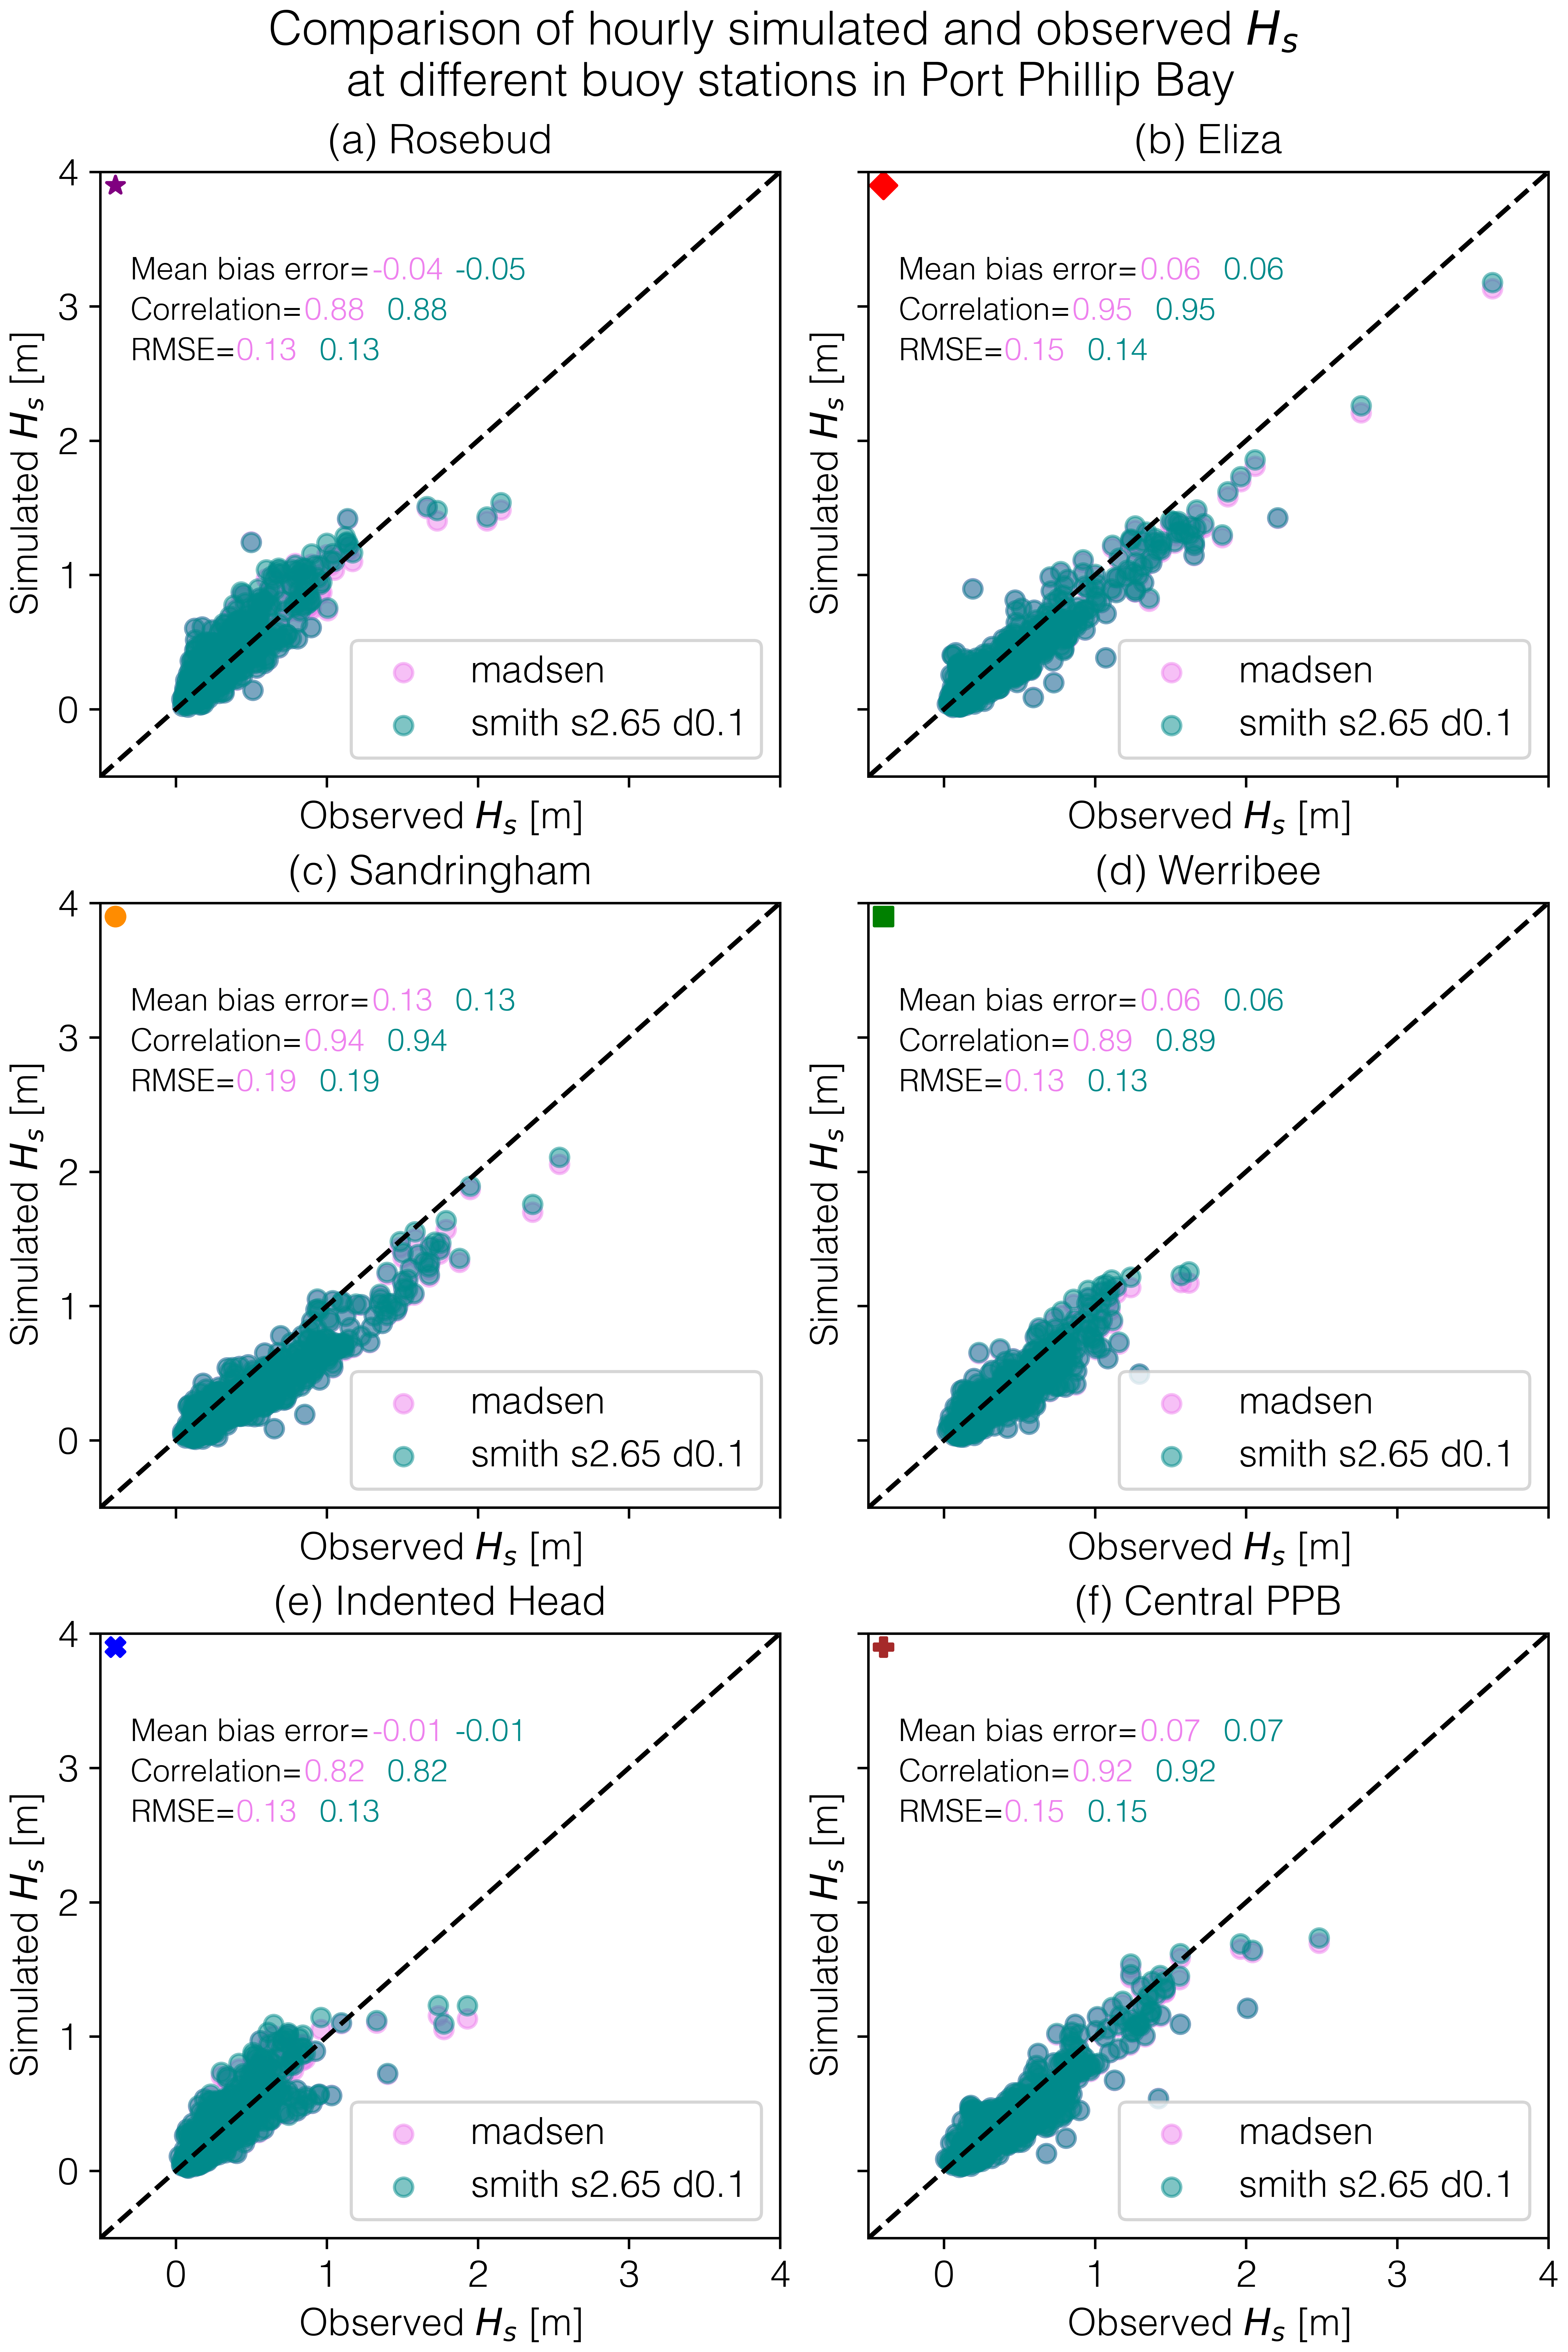
\includegraphics[scale=0.7]{plots/scatter/madsen_vs_smith s2.65 d0.1_vert_sca.png}
    \caption{Comparison between modelled and observed $H_{s}$ values for each buoy for the experiments: madsen (pink dots) and smith s2.65 d0.1 (cyan dots) }
    \label{fig:scatter_madsen_vs_smith_def}
\end{figure}

The differences between the experiments at the peaks do not have a strong influence in the skill metrics of the model as it presented in the scatter plots. The only change happens in the RMSE values for the Mt Eliza station where the \textbf{smith s2.65 d0.1} experiment has a value of 0.14 while \textbf{madsen} experiment has 0.15. Sandringham is the station with the largest positive bias which indicates an systematic $H_s$ underestimation. \textcolor{red}{statement about smith better than madsen}.\\

The following experiment is smith s2.65 d0.78 which employs a more realistic diameter grain size of 0.78mm for the bay because is computed as the mean value for the entire area according to the dataset. This experiment is compared with \textbf{smith s2.65 d0.1} to establish a comparison about how the changes on the diameter grain size can affect the estimation of $H_s$ for the simulation period. The $H_s$ series are presented below.

\begin{figure}[H]
    \centering
    \includegraphics[scale=0.7]{plots/hs_series/smith s2.65 d0.1_vs_smith s2.65 d0.78_vert.png}
    \caption{$H_{s}$ time series for each buoy under smith s2.65 d0.1 (cyan line) and smith s2.65 d0.78 (orange line) experiments.}
    \label{fig:hs_smith_def_vs_smith_0.78}
\end{figure}

The largest $H_s$ values for each station are better estimated by \textbf{smith s2.65 d0.1} than \textbf{smith s2.65 d0.78}, but the differences are not larger than 0.03 m. This behaviour is quite reasonable based on the fact that ... \textcolor{red}{statement about why larger diameters can increase bottom friction dissipation}.

\begin{figure}[H]
    \centering
    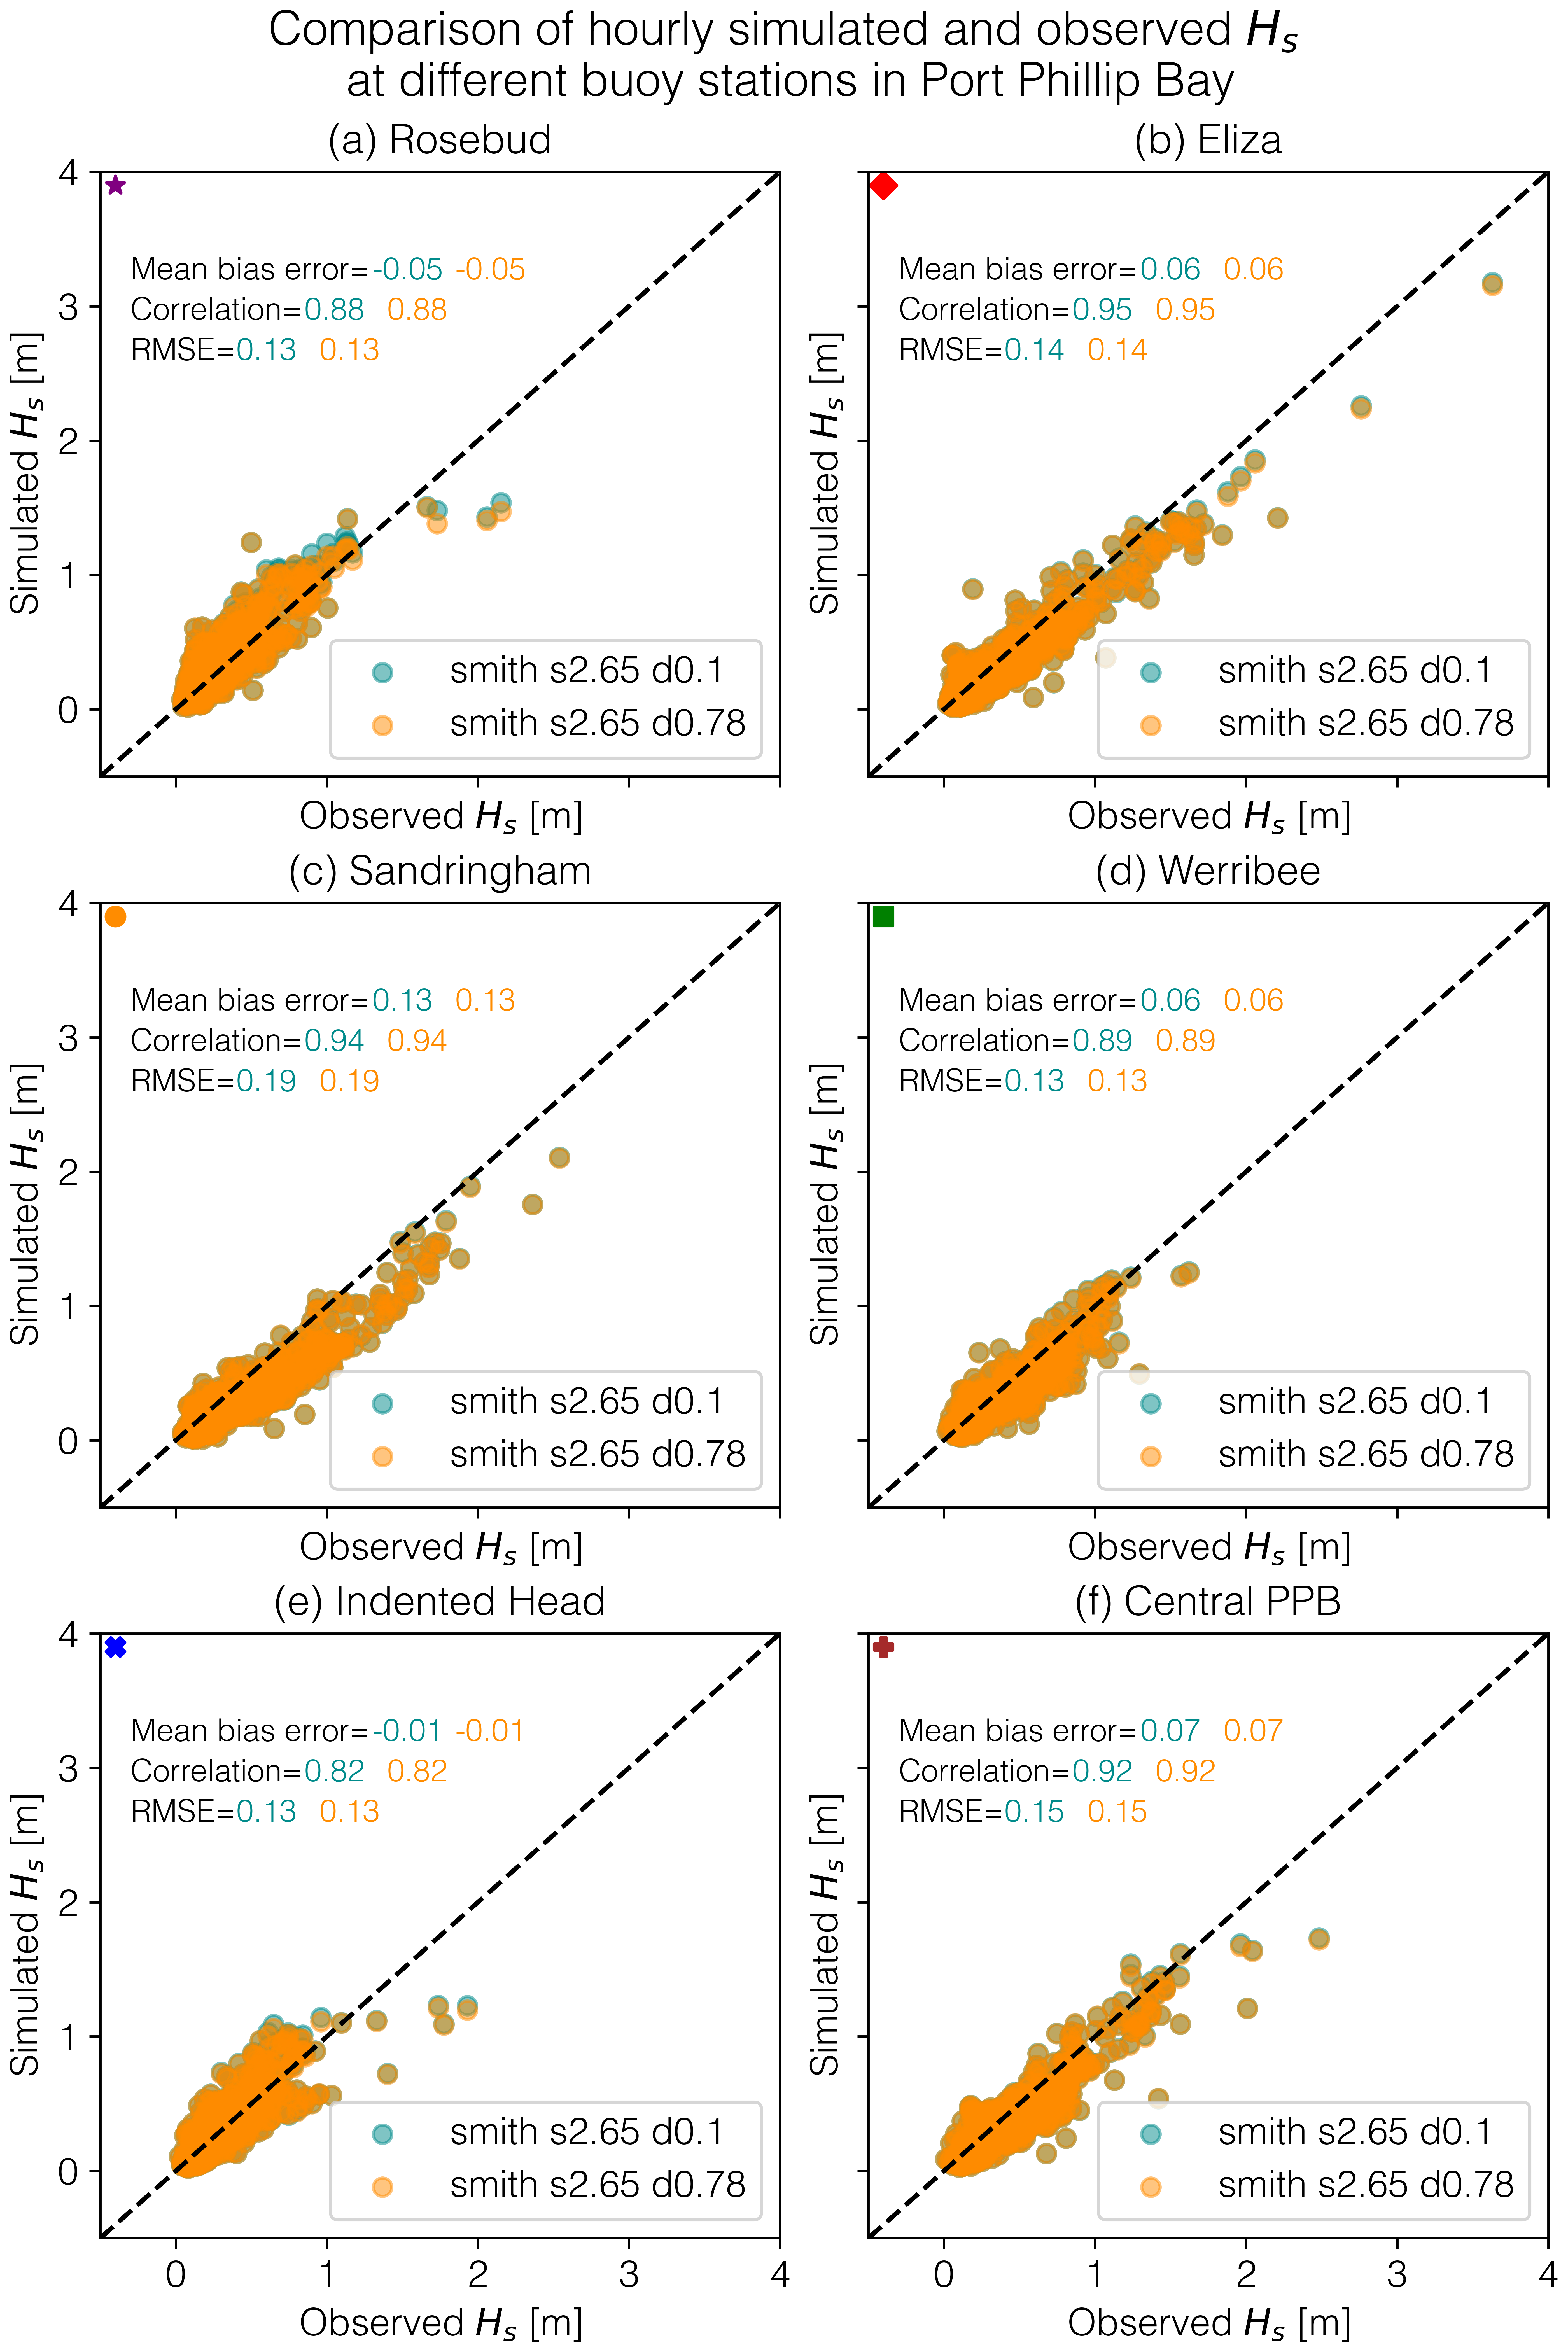
\includegraphics[scale=0.7]{plots/scatter/smith s2.65 d0.1_vs_smith s2.65 d0.78_vert_sca.png}
    \caption{Comparison between modelled and observed $H_{s}$ values for each buoy for the experiments: smith s2.65 d0.1 (cyan dots) and smith s2.65 d0.78 (orange dots)}
    \label{fig:scatter_smith_def_vs_smith_0.78}
\end{figure}

The changes are not enough strong to modify the model skills when the experiments are compared throughout the scatter plots and 4 out of 6 stations (Sandringham, Werribee, Mt Eliza and Central PPB) show an overall underestimation. All the mean bias error (MBE), the correlation and the root mean squared error (RMSE) are identical for all the stations. Although the last experiment uses a most representative diameter grain size for the bay, the ideal scenario should be the inclusion of the spatial variability of the diameter across PPB because the dataset clearly shows that there is a range of variation from 0.3 to 1 mm (see fig. \ref{fig:diameter_PPB}). Another experiment is then tested using this new inclusion: \textbf{smith s2.65 dvar}.

\begin{figure}[h]
    \centering
    \includegraphics[scale=0.7]{plots/hs_series/smith s2.65 d0.78_vs_smith s2.65 dvar_vert.png}
    \caption{$H_{s}$ time series for each buoy under smith s2.65 d0.78 (orange line) and smith s2.65 dvar (red line) experiments.}
    \label{fig:hs_smith_0.78_vs_smith_dvar}
\end{figure}

\textbf{smith s2.65 dvar} and \textbf{smith s2.65 d0.78} were compared to evaluate the effect of a most realistic diameter grain size information in the model. Despite the generation of the sediment diameter map, the largest $H_s$ values for each station barely increase between 0.01 and 0.03 m as it is depicted in the figure XX. Stations like Sandringham still shows a systematic underestimation of the $H_s$ values and the maximum modelled $H_s$ value is still 0.5 m under the observation. 

\begin{figure}[H]
    \centering
    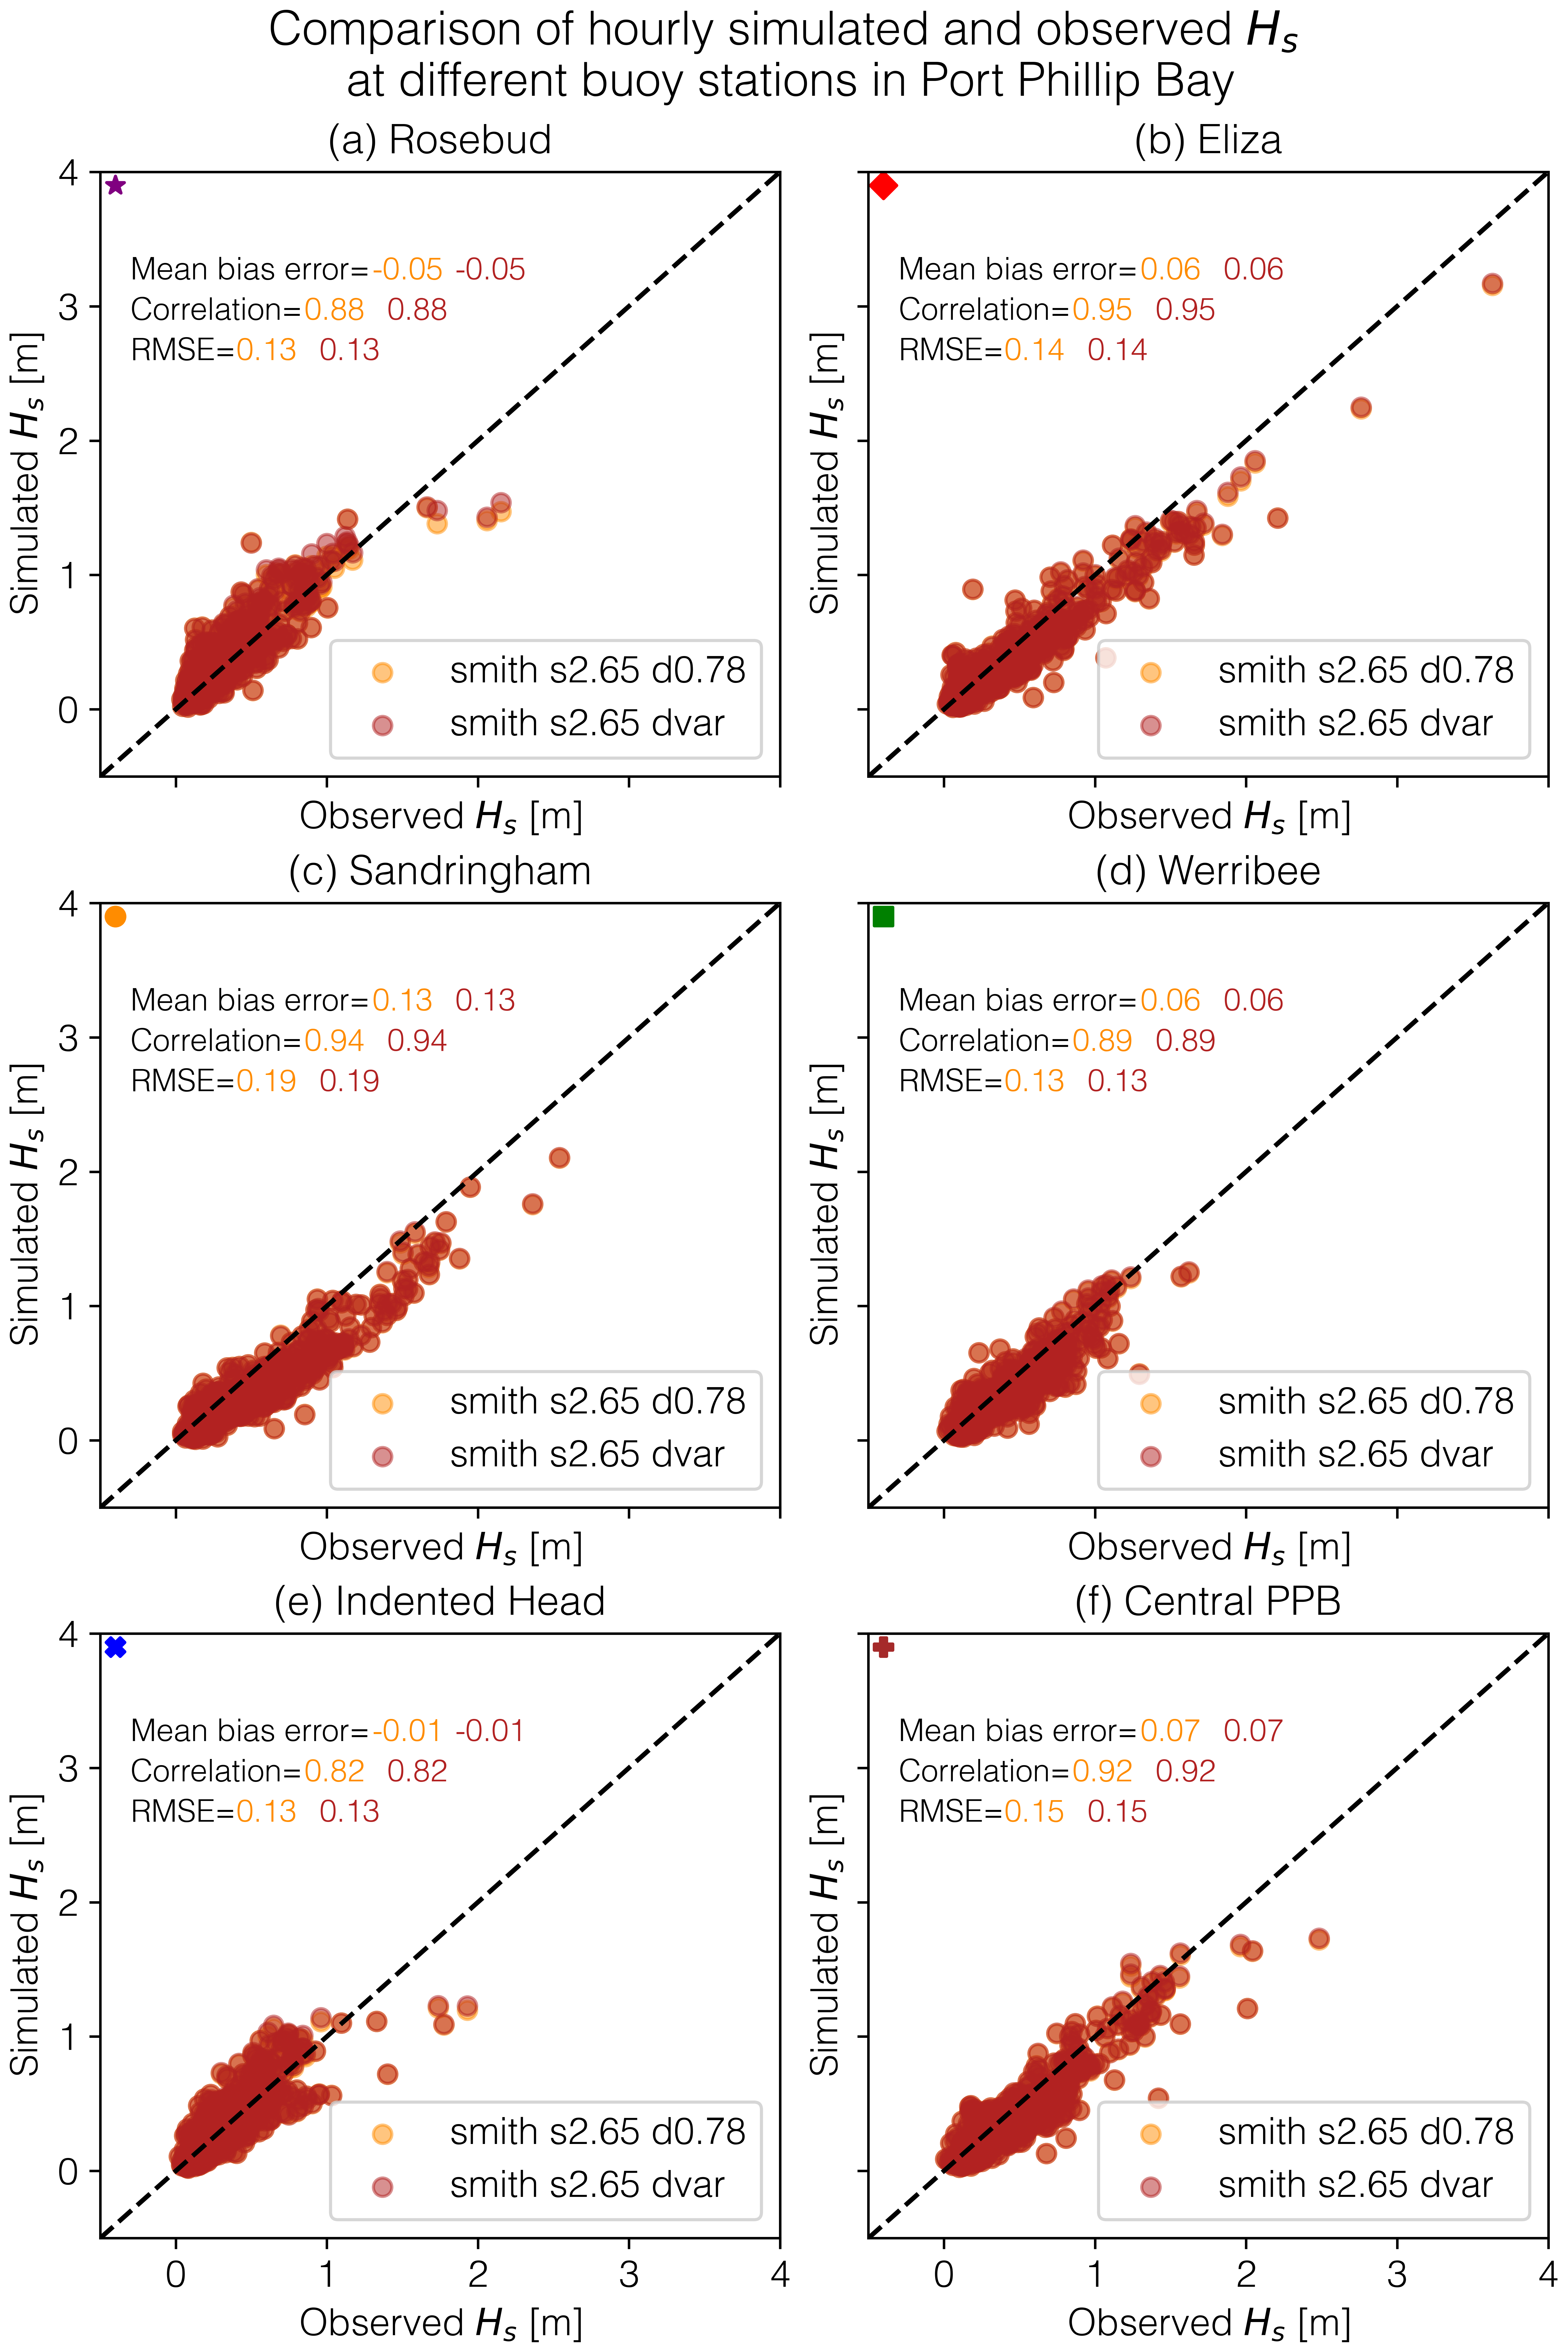
\includegraphics[scale=0.7]{plots/scatter/smith s2.65 d0.78_vs_smith s2.65 dvar_vert_sca.png}
    \caption{Comparison between modelled and observed $H_{s}$ values for each buoy for the experiments: smith s2.65 d0.78 (orange dots) and smith s2.65 dvar (red dots)}
    \label{fig:scatter_smith_0.78_vs_smith_dvar}
\end{figure}

The scatter plots are identical than those ones presented in the figure \ref{fig:scatter_madsen_vs_smith_def}, and any change on the skill metrics are evidenced. These results were suspicious due to the error metrics did not change at all and the largest $H_s$ values modelled with \textbf{smith s2.65 dvar} are identical to those ones obtained with \textbf{smith s.265 d0.1}. It was highly possible that SWAN was not reading the sediment diameter map and it was just applying the default conditions for the \textcite{Smith2011} parametrization. A further look in the source code exhibits that in the file \verb|swanmain.ftn| the following conditional is written in the lines 3722-3726:

\begin{lstlisting}[language=Fortran]
IF (VARFR .AND. IBOT.EQ.5) THEN                                 41.51
     CALL MSGERR (1,
 &           'Ripples model active, space varying friction ignored')
     VARFR = .FALSE.
ENDIF
\end{lstlisting}

Where \verb|IBOT| is an indicator for the bottom friction which is specified in the file \verb|swancom.ftn|

\begin{lstlisting}[language=Fortran]
!     IBOT              Indicator for bottom friction
!                       IBOT = 0  no bottom friction dissipation
!                       IBOT = 1  Jonswap bottom dissipation model
!                       IBOT = 2  Dingemans bottom dissipation model
!                       IBOT = 3  Madsen bottom dissipation model
!                       IBOT = 5  bottom dissipation due to ripples
\end{lstlisting}
      
Finally, a last experiment was made to evaluate a most physical specific gravity for the bay. The default value is 2.65 based on the original parametrization, but based on the predominance of sublitoral mud, a most representative value for PPB would be 2.75. This value was tested in the experiment \textbf{smith s2.75 d0.01} and it was compared with \textbf{smith s2.65 d0.01}. The $H_s$ variability looks exactly identical for both simulations and the largest $H_s$ modelled values are the same. 

\begin{figure}[H]
    \centering
    \includegraphics[scale=0.7]{plots/hs_series/smith s2.65 d0.01_vs_smith s2.75 d0.01_vert.png}
    \caption{$H_{s}$ time series for each buoy under smith s2.65 d0.01 (blue line) and smith s2.75 d0.01 (green line) experiments.}
    \label{fig:hs_smith_s2.65_vs_smith_s2.75}
\end{figure}

The scatter plots end up showing the same distribution of the measured and modelled $H_s$ values for both experiments. This confirms that the changes on the specific gravity do not imply a strong effect in the estimation of $H_s$ values for PPB and the $H_s$ estimations can not be improved neither.

\begin{figure}[H]
    \centering
    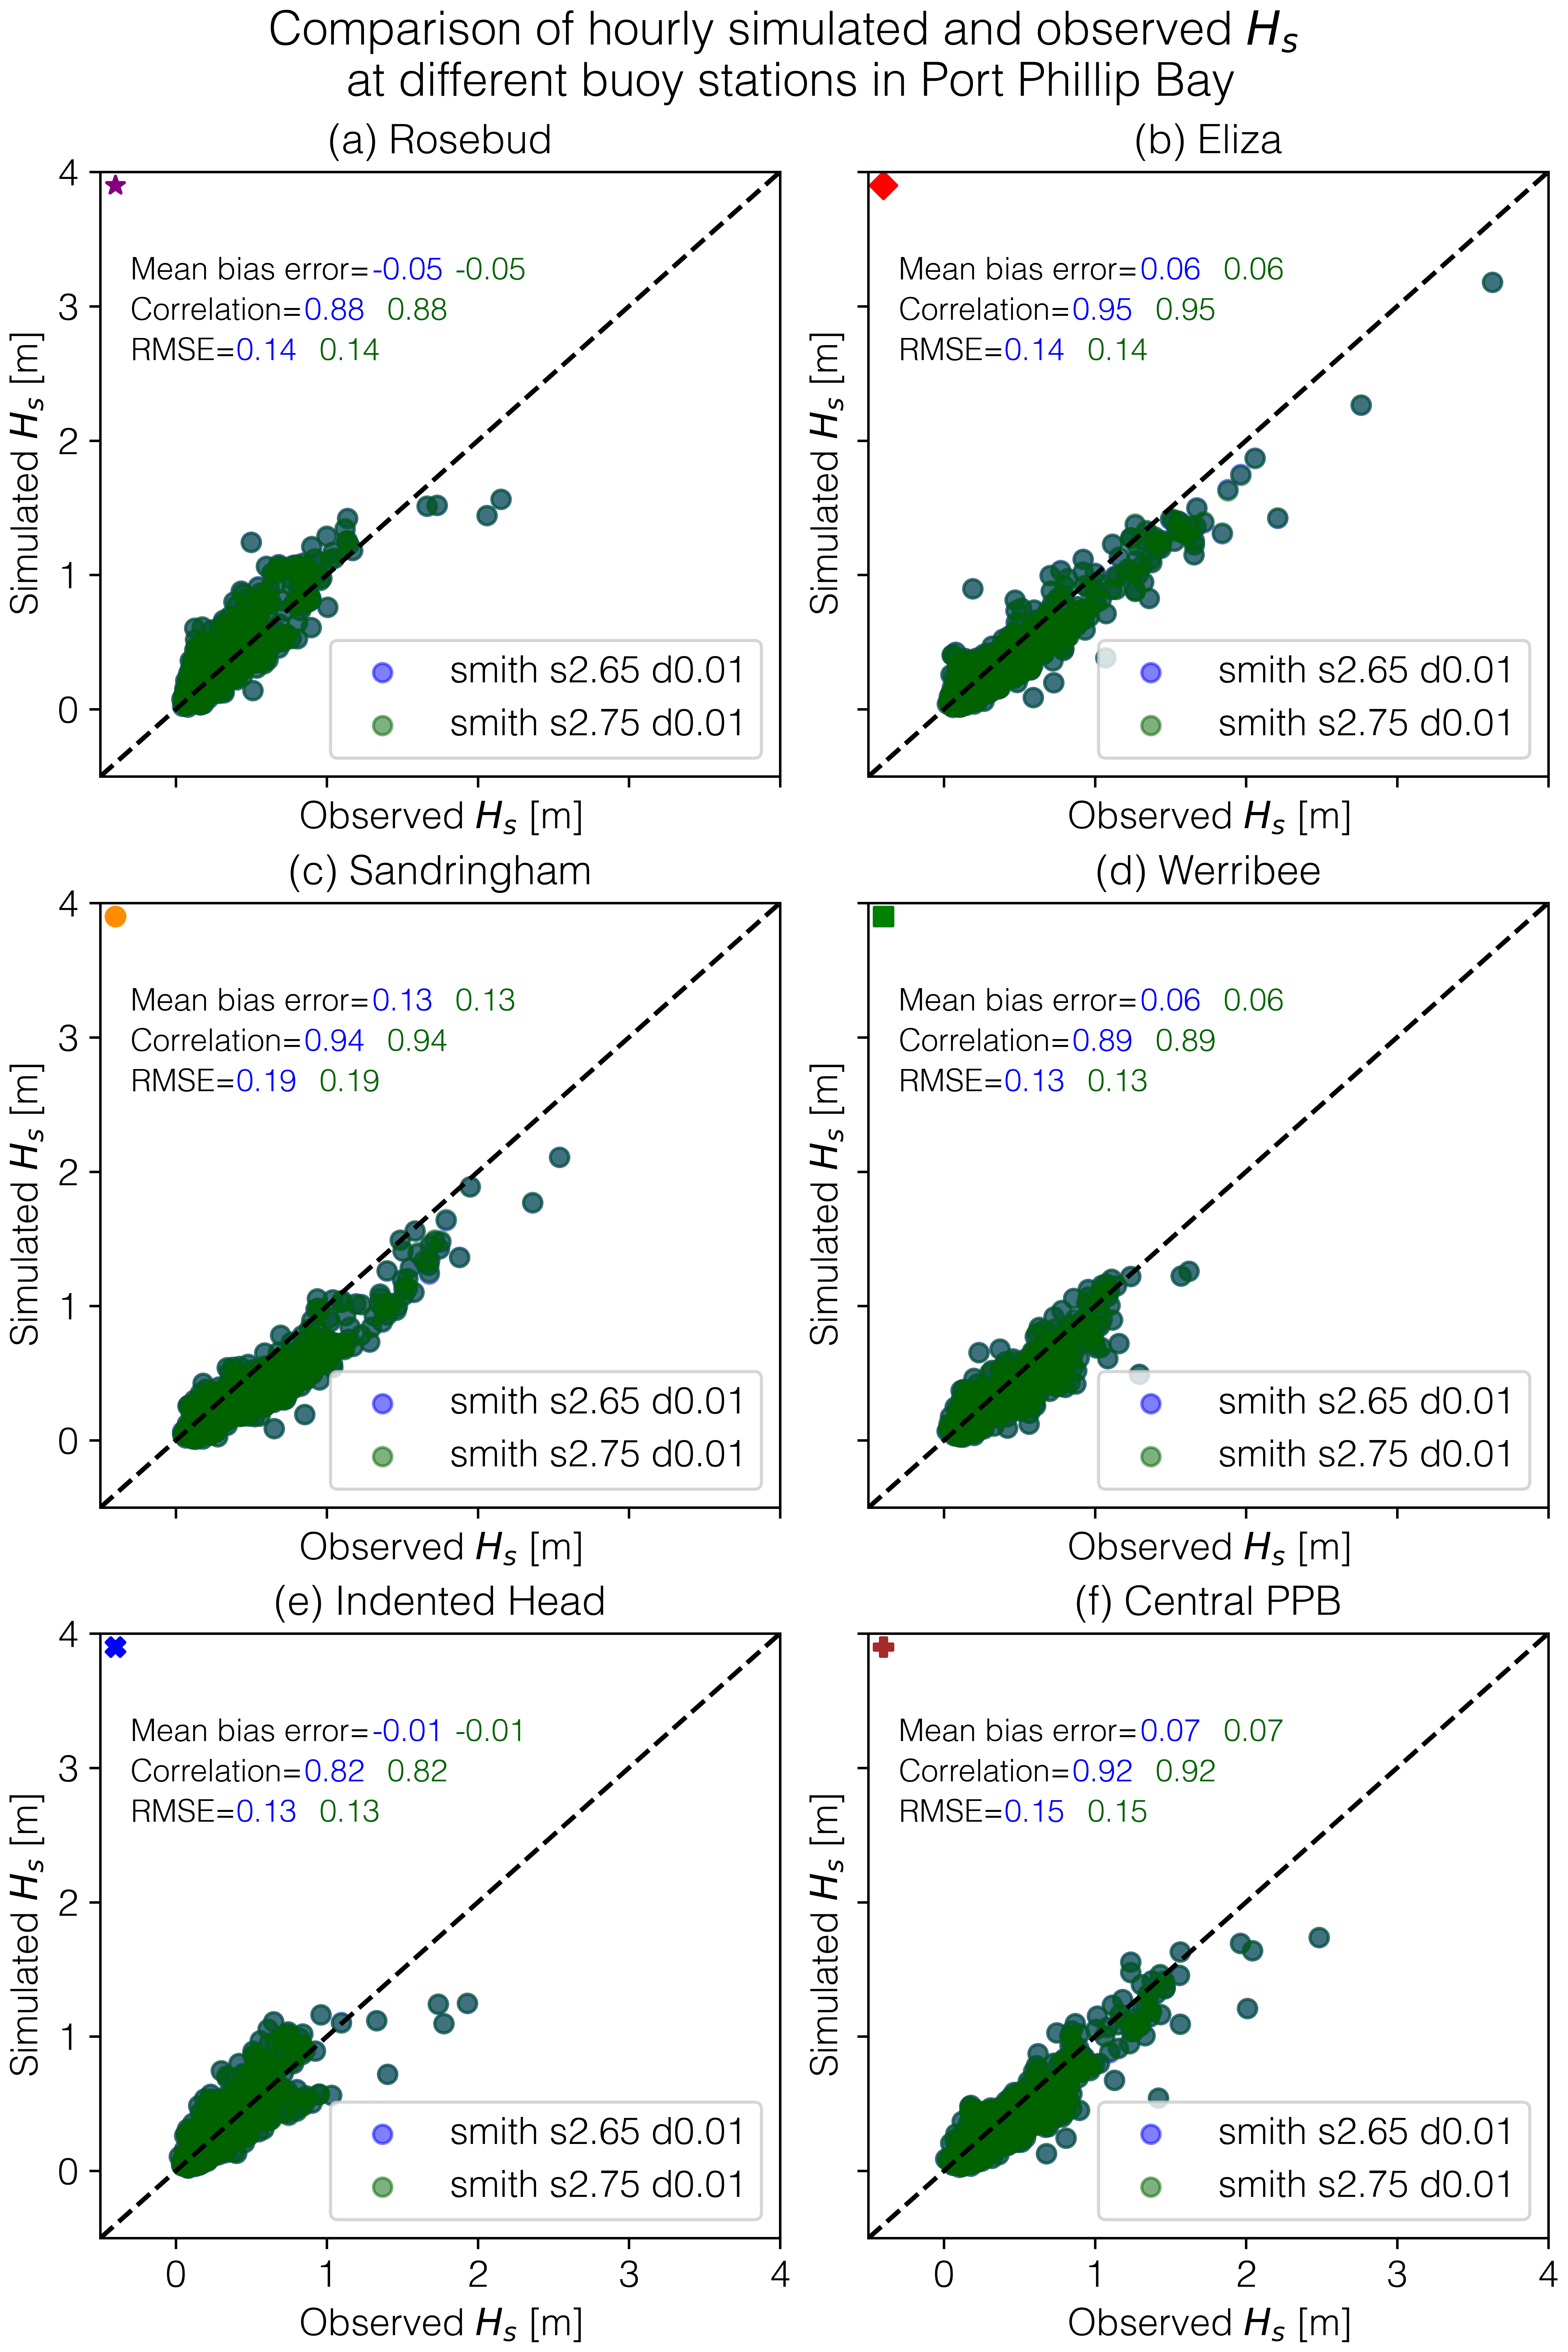
\includegraphics[scale=0.7]{plots/scatter/smith s2.65 d0.01_vs_smith s2.75 d0.01_vert_sca.png}
    \caption{Comparison between modelled and observed $H_{s}$ values for each buoy for the experiments: smith s2.65 d0.01 (blue dots) and smith s2.7 d0.01 (green dots)}
    \label{fig:scatter_smith_s2.65_vs_smith_s2.75}
\end{figure}

As long as smith parametrization in SWAN does not include spatial variability of diameter grain size and specific gravity, a most realistic scenario for the wave modelling in PPB can not be tested and the best configuration that can be used is \textcolor{red}{XXYYZZ}. 

\section{Simulation results including vegetation}

\subsection{A vegetation test case}

Initially, the vegetation test case for COAWST was simulated to verify the correct performance of the vegetation module and its interaction with SWAN and ROMS \parencite{Beudin2017}. A description and a scheme of the test case is presented below 

\begin{figure}[H]
    \centering
    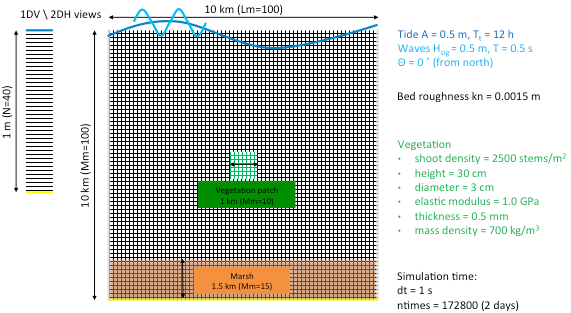
\includegraphics[scale=0.6]{plots/vegetation_test.png}
    \caption{}
    \label{fig:}
\end{figure}

It is worth to mention that the southern edge is closed (zero gradient condition) and the western and eastern sides have a zero gradient boundary condition for the flow and an absorbing condition for the wave energy. \textcite{Beudin2017} demonstrated the effect of vegetation patch on the middle of the domain throughout the depth-averaged velocity at peak flood as it shown in figure \ref{fig:depth_avg_vel_1}

\begin{figure}[h]
\centering
\begin{subfigure}{.5\textwidth}
  \centering
  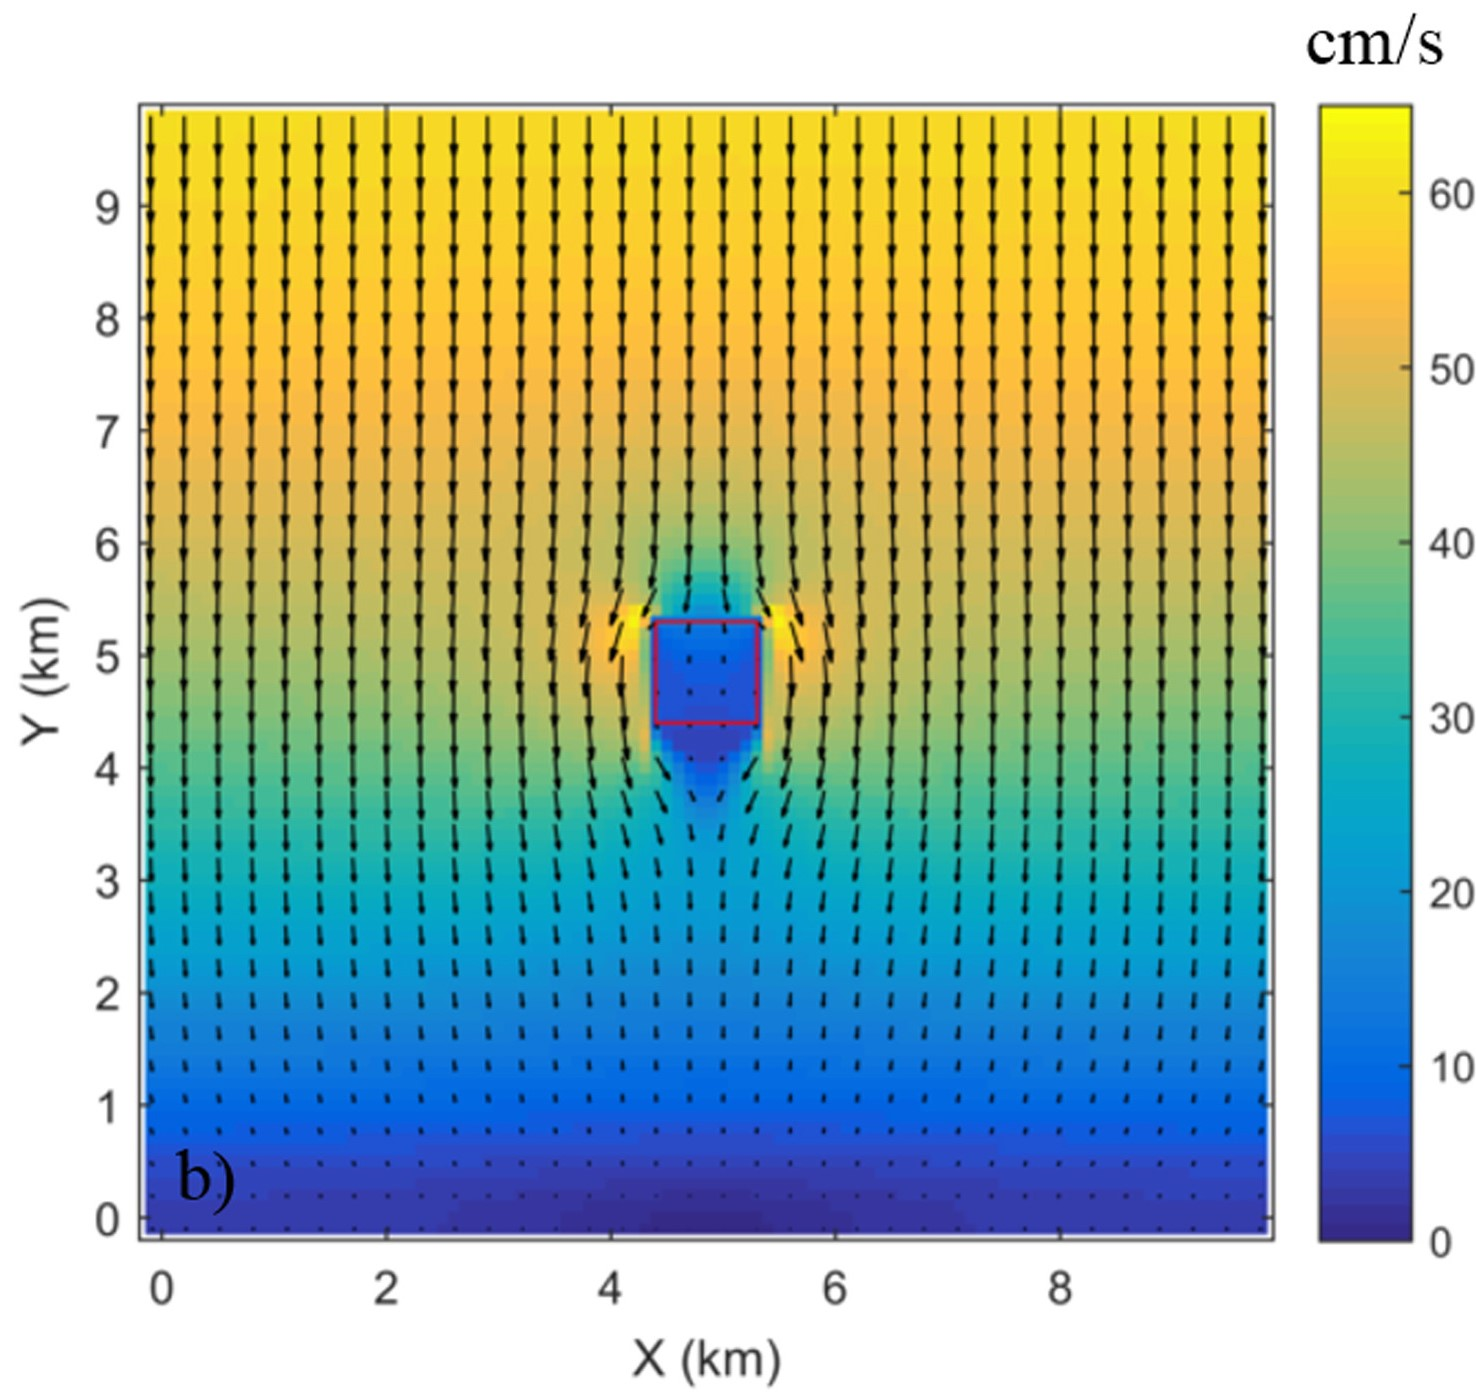
\includegraphics[scale=0.17]{plots/depth_averaged_vel_full.jpg}
  \caption{Depth-averaged velocity, at peak flood presented in \textcite{Beudin2017}}
  \label{fig:depth_avg_vel_1}
\end{subfigure}%
\begin{subfigure}{.5\textwidth}
  \centering
  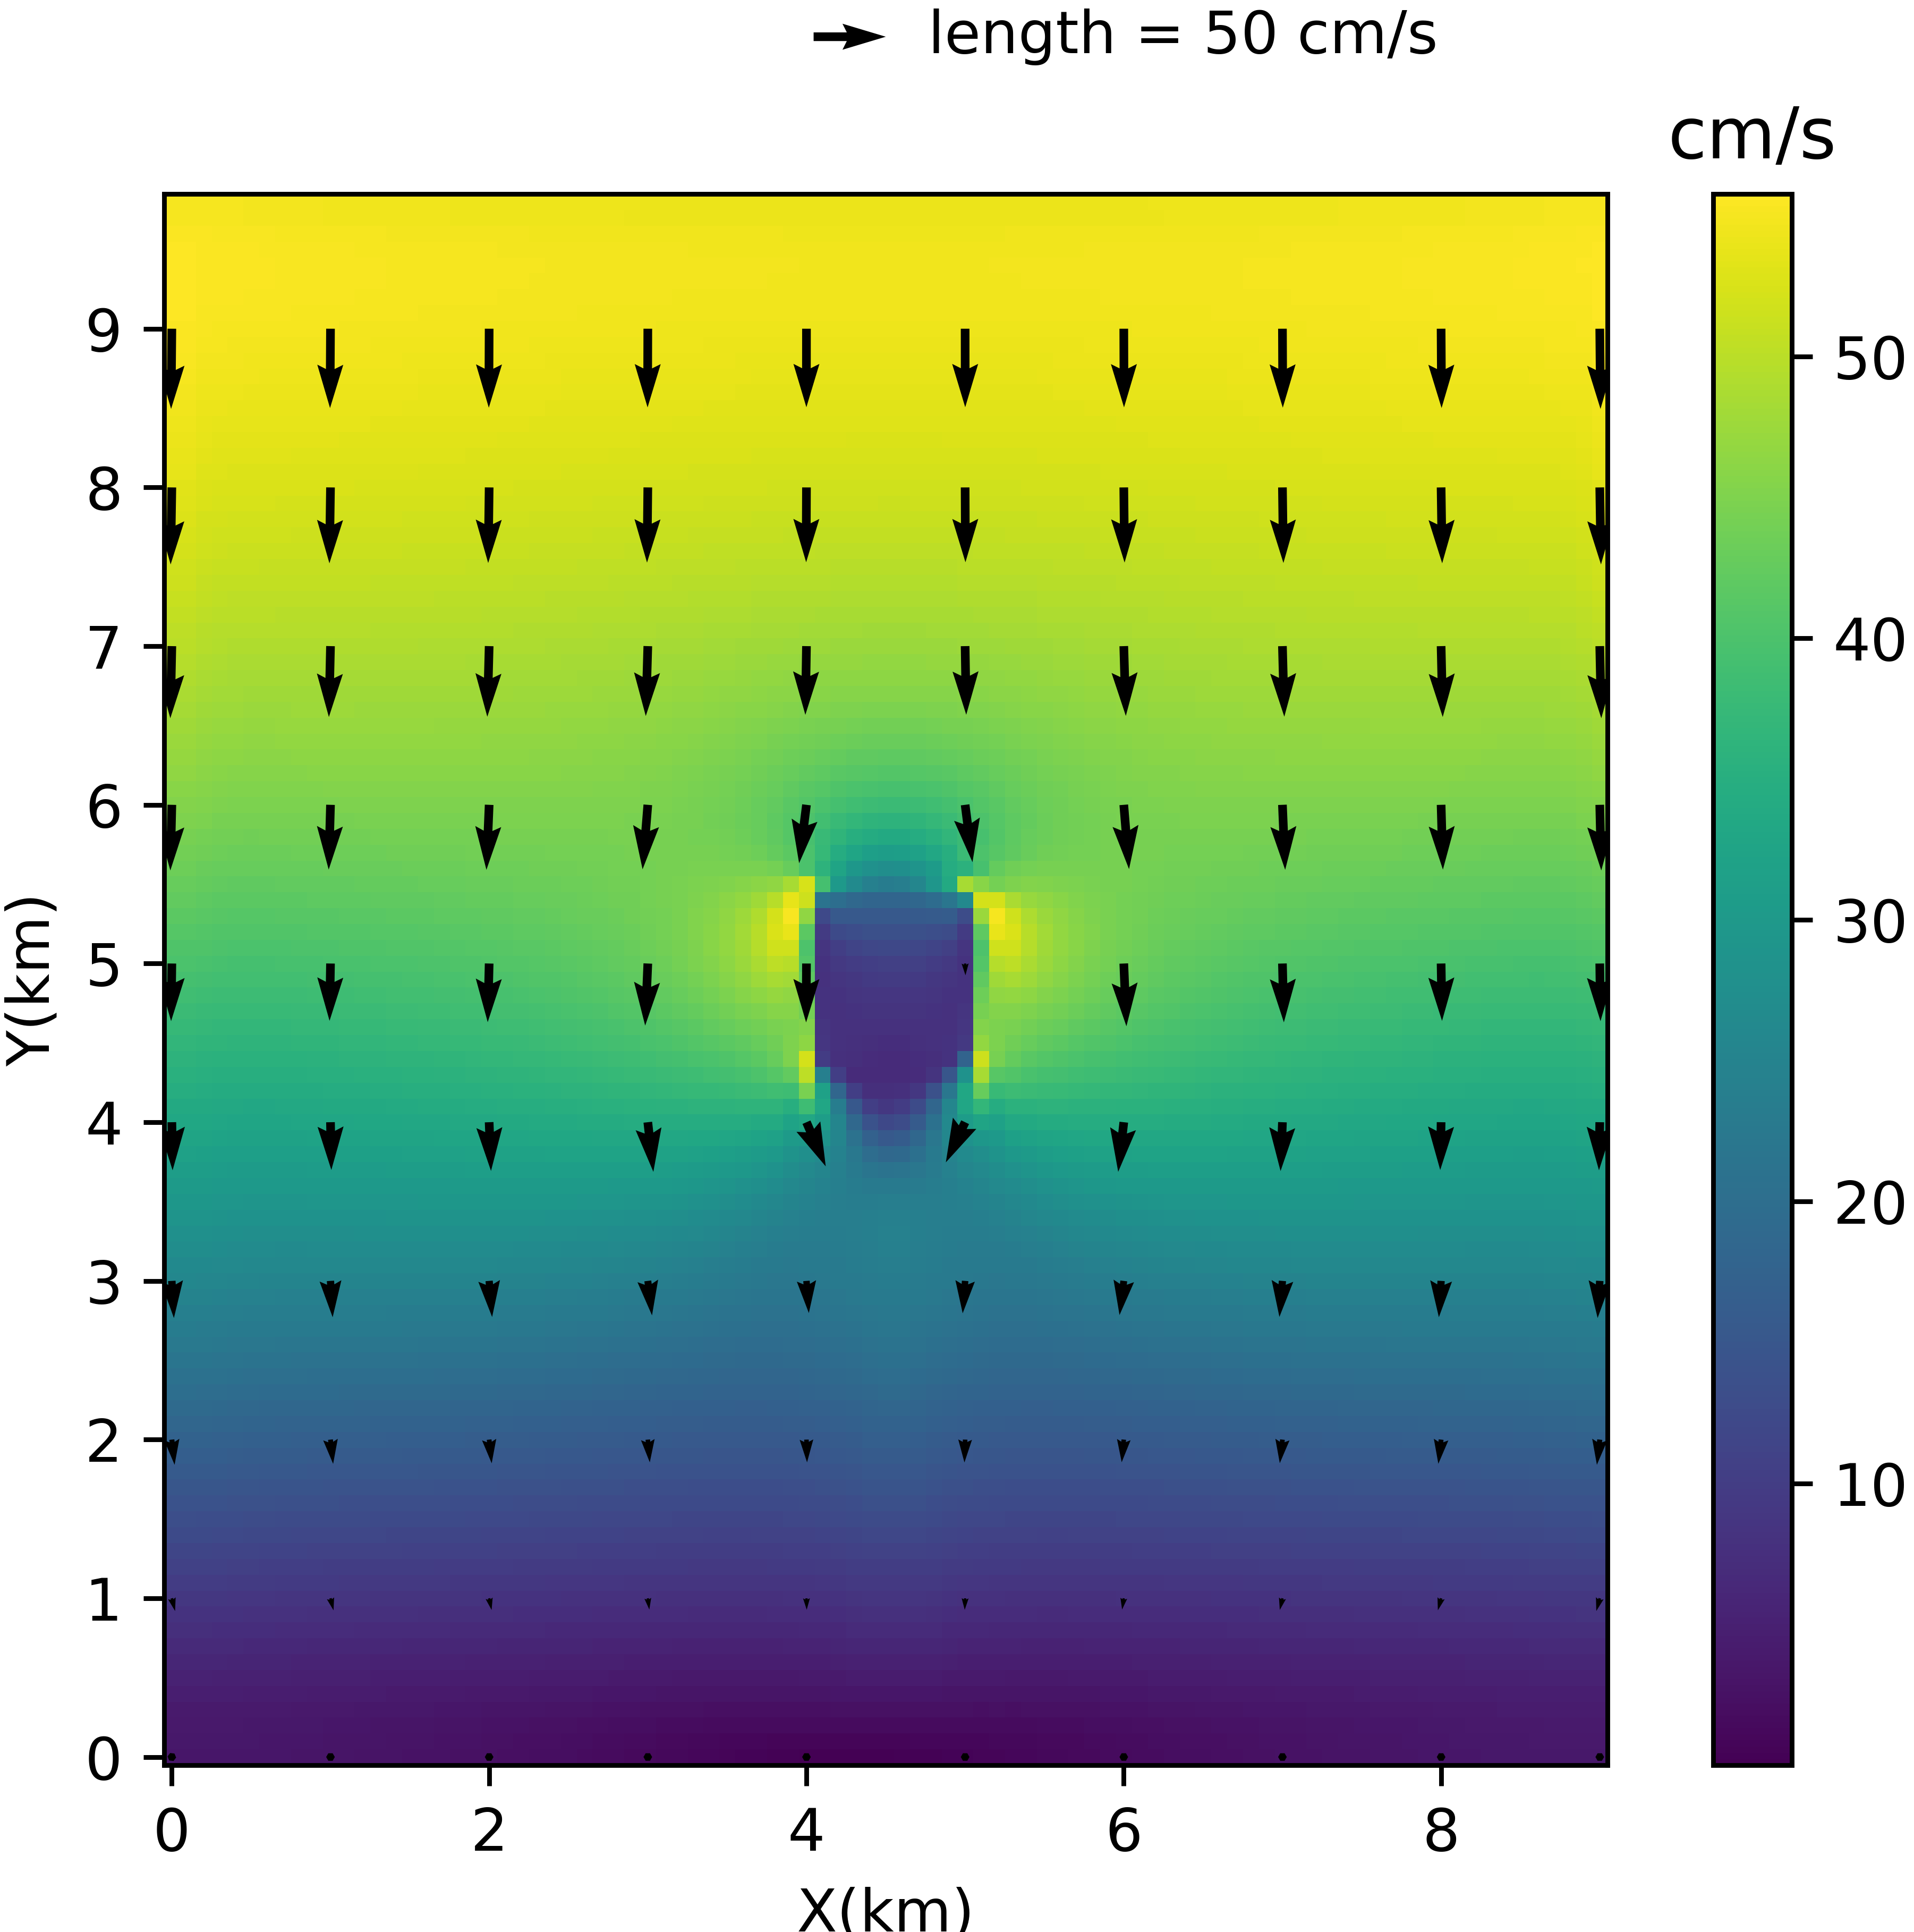
\includegraphics[scale=0.55]{plots/depth_averaged_vel_veg_test.png}
  \caption{Depth-averaged velocity, at peak flood computed with the configured model}
  \label{fig:depth_avg_vel_2}
\end{subfigure}
\caption{Comparison of the depth-averaged velocities, at peak flood according to the results evidenced by \textcite{Beudin2017} and those ones obtained with our verification of the test case. The patch of (stiff) vegetation is located in the red square. The hydrodynamic is forced at the northern boundary.}
\label{fig:grid_bathy_PPB}
\end{figure}

\subsection{An idealized case}

\section{Conclusions and recommendations}

This report summaries the work done in Stage 1 of the Wave-Hydrodynamic Modelling research project funded by the Department of Energy, Environment and Climate Action (DEECA). It focuses on updating the PPB wave-ocean hindcast datasets  for 5 different SLR scenarios (0.0 m, 0.5 m, 0.8 m, 1.1 m and 1.4 m) to 32 years outputted for every hour (hourly interval) using the state of the art wave physics (ST6) and the newly ERA5 atmospheric forcing field with the wind field locally adjusted to optimise the wave model performance which was validated against the operational wave buoy network recently deployed within the Bay.  
Although every effort has been made to produce a high quality hindcast dataset up to present time, it is believed that a new version of this dataset will be made available when there is a new or an improved atmospheric product released to the public (e.g. ERA6). Other organisations who wished to use this dataset should contact DEECA for the data permission and the University of Melbourne for a consultation and guidance. 

% \textcolor{red}{The PPB is arguably one of the most important environmental, social and economic asset in Victoria. Most of the population that lives near coastal areas in PPB could be exposed to coastal erosion and flooding hazards induced by sea level rise. An unstructured grid coupled modelling system SCHISM-WWMII is purposed and configured to evaluate the effect of different sea level change scenarios on the shoreline dynamic with a high-resolution mesh used to capture the complex coastal shoreline and bathymetry in PPB. Additionally, a real-time buoy network has been deployed to monitor wave variables in PPB with the aim of calibrating and validating the aforementioned coupled modelling system. Calibration and validation processes have shown an overall good agreement between the modelled values and the SWH values recorded by most of the buoys. Werribee, Central PPB, and Indented Head stations show overestimations of the higher $H_{s}$ values recorded during the simulation period, while underestimation of SWH peak values during a storm in Mt. Eliza station was recorded in late October. It was corrected by a local wind scaling. A configuration with no wind forcing and regional wind scaling showed the best agreement with the buoy measurements. This modelling system was then used to simulate five different sea level hindcast scenarios and the results are prepared to build the probability distribution of the extreme $H_{s}$ and sea level values.}

\newpage
\section*{Acknowledgements}

This study was funded by Department of Energy, Environment and Climate Action (DEECA) through Port Phillip Bay Beach Renourishment Program. Hindcast simulations and post-data processing were undertaken on supercomputer systems within the University of Melbourne and the National Computational Infrastructure (NCI), including Spartan and GADI.

\newpage
\printbibliography

\newpage
\end{document}
